
%\special{papersize=8.5in,11in}
%\documentclass[titlepage,12pt] {article}  
%\usepackage{setspace}
%\topmargin =-1.5cm \evensidemargin = -0.02in
%\oddsidemargin=-0.02in \textwidth=16.5cm \textheight=24cm
%\usepackage{fullpage}

\documentclass[sn-mathphys,Numbered, super, referee, lineno]{sn-jnl}
%\documentclass[sn-nature,Numbered, super]{sn-jnl}

\usepackage[nolists, fighead]{endfloat}

\renewcommand{\efloatseparator}{\mbox{}}

\usepackage{color}
\usepackage{array}
\usepackage{natbib}
\usepackage{graphics}
\usepackage{graphicx}
\usepackage{amsmath,amssymb,amsfonts}
\usepackage{amsthm}
\usepackage{mathrsfs}
\usepackage{epsfig}
\usepackage[title]{appendix}
\usepackage{alltt}
\usepackage{textcomp}
\usepackage{multirow}
\usepackage{hyperref}
\usepackage{physics}
\usepackage{xcolor}
%\usepackage{caption}
%\usepackage{subcaption}
\usepackage{textcomp}%
\usepackage{manyfoot}%
\usepackage{booktabs}%
\usepackage{algorithm}%
\usepackage{algorithmicx}%
\usepackage{algpseudocode}%
\usepackage{listings}
\usepackage{chngcntr}
\renewcommand{\arraystretch}{1.5}


%\newcolumntype{L}[1]{>{\raggedright\let\newline\\\arraybackslash\hspace{0pt}}m{#1}}

%\newcommand{\beginsupplement}{%
%        \setcounter{table}{0}
%        \renewcommand{\thetable}{S\arabic{table}}%
%        \setcounter{figure}{0}
%        \renewcommand{\thefigure}{S\arabic{figure}}%
%     }


\begin{document}

\title[Article Title]{The response time paradox in functional magnetic resonance imaging analyses}

\author*[1]{\fnm{Jeanette A.}  \sur{Mumford}}\email{jeanette.mumford@gmail.com}

\author[1]{\fnm{Patrick G.} \sur{Bissett}}
\author[2]{\fnm{Henry M.} \sur{Jones}}
\author[1]{\fnm{Sunjae} \sur{Shim}}
\author[1]{\fnm{Jaime Ali H.} \sur{Rios}}
\author[1]{\fnm{Russell A.} \sur{Poldrack}}
\affil[1]{Department of Psychology, Stanford University, Stanford, CA, United States of America}
\affil[2]{Department of Psychology, University of Chicago, Chicago, IL, United States of America}



\abstract{Response times (RTs) are often the main signal of interest in cognitive psychology, but are often ignored in functional MRI (fMRI) analyses.  In fMRI analysis the intensity of the signal serves as a proxy for the intensity of local neuronal activity, but changes in either intensity or duration of neuronal activity can yield identical fMRI signals.  Therefore, if RTs are ignored and pair with neuronal durations, fMRI results claiming intensity differences may be confounded by RTs. We show how ignoring RTs goes beyond this confound, where longer RTs are paired with larger activation estimates, to lesser-known issues where RTs become confounds in group-level analyses and, surprisingly, how the RT confound can induce other artificial group-level associations with variables that are not related to the condition contrast or RTs.  We propose a new time-series model to address these issues and encourage increasing focus on what the widespread RT-based signal represents.} 




\maketitle

\section*{Introduction}

The goal of task-based functional magnetic resonance imaging (fMRI) studies is to infer involvement of particular brain regions or networks in specific cognitive functions.  These studies are often designed using the subtraction logic first developed by \citet{donders1969} for the analysis of response times (RTs), in which comparisons are made between different task conditions thought to differ with regard to involvement of some specific cognitive function(s).  For example, in the well-known Stroop task, stimuli are presented where color and text of words are either congruent (e.g.\, ``blue" presented in blue) or incongruent (e.g.\, ``blue" presented in red) \citep{stroop_1935}.  Individuals are consistently slower at naming stimulus color when the written word is incongruent compared to congruent, and this difference in response times is interpreted as indexing engagement of an additional cognitive process in the incongruent condition, such as conflict detection or resolution \citep{botvinick2001}. Similarly, greater activation in regions such as the dorsal medial frontal cortex (dMFC) in fMRI studies of the Stroop task have been interpreted as reflecting a specific role in these cognitive processes \citep{botvinick1999, macdonald2000, kernsAnteriorCingulateConflict2004}.  

The facile nature of the common inference from activation to ``involvement'' belies the complexity of the link between fMRI signals and underlying neuronal activity (cf. \citet{logothetisWhatWeCan2008}).  Here we focus on disambiguating these interpretations of activation: namely, whether a difference in activation reflects differential engagement of a particular computation, or engagement of the same computation for a different amount of time.  Because of the slow nature of the blood oxygen-level dependent (BOLD) response, measured in most fMRI studies, it is difficult to distinguish the degree to which a difference in evoked BOLD response reflects an increase in amplitude of neuronal response versus a difference in response duration (Figure \ref{fig:neuron_bold}).  This indeterminacy has been known since the early days of fMRI \citep{savoy1995, fslbook2001} and establishes the importance of considering the potential for differences in duration of neural activity to confound amplitude estimates in some fMRI tasks.  

For clarity, we define some terms used throughout the present paper. Time-series level analysis refers to linear models of fMRI time-series. Group-level analyses refer to analyses of estimated fMRI contrasts across a set of subjects including a single group average (1-sample t-test), group average comparisons (2-sample t-test) and linear associations with a covariate (e.g., phenotype).  Between-trial RT adjustment is formally carried out in the time-series level. Between-subject RT confounds will only impact group-level models involving group comparisons or associations but not single group averages.  

Over a decade ago,  \citet{grinband_detection_2008} started the discussion about between-trial modeling of response times in fMRI analysis.  They proposed a variable epoch model, where trial-by-trial neuronal durations were assumed to track with RTs as opposed to a common modeling practice that assumed each trial was sufficiently modeled as a brief impulse of constant duration (e.g., .1s).  The impulse model was  considered to be adequate due to the belief that differences in RTs would not be detectable. The variable epoch model yielded more powerful results than the impulse model or an impulse model with an RT-modulated regressor.  Importantly, this model's performance studied within-subject power for a single condition versus baseline and assumed the neuronal activation duration mirrors the RTs.  The assumption that neural activity duration scales with RT may be particularly suitable when the neural signature is theoretically linked to the accumulation of information towards a response, as in the accumulation of activity towards a response in the Diffusion Decision Model \citep{ratcliff1978}. There are likely tasks and regions of the brain for which this assumption and therefore this modeling strategy is appropriate, but this is a strong theoretical commitment that may not be suitable for all tasks or for the whole brain. How this model performs for condition differences and when model assumptions are violated has not been well studied.   

\citet{yarkoni_bold_2009} examined the relationship between RT and fMRI signal across a variety of tasks in an effort to better understand how RTs were related to BOLD signal amplitude.  RT-driven amplitude differences were found to be due to ``time on task'' or simply duration differences in the neuronal signal across trials (constant activity that varies in duration), as opposed to differences in the magnitude of neuronal activity.    A compelling result of this work was the identification of a widespread network of brain regions that showed significant correlation with RTs across  a variety of  tasks including the dMFC which was previously described as reflecting conflict in the Stroop task.  This calls into question how RT-based activation differences might be interpreted given they are present across many tasks.

\begin{figure}[!ht]
  \centering
%   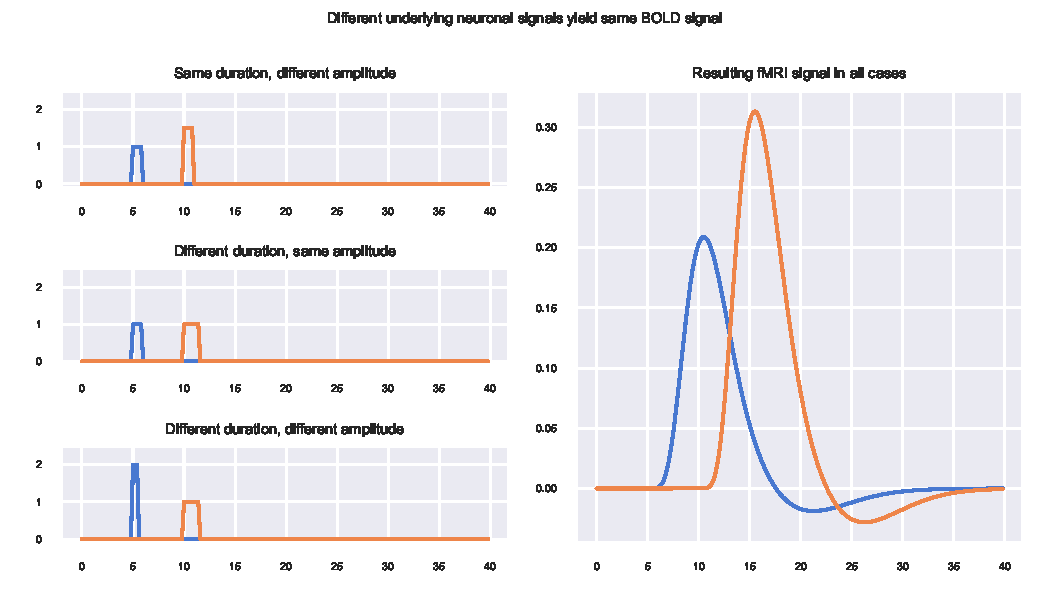
\includegraphics[width=\linewidth]{fig1_neuron_same_bold.pdf}
   \caption{How amplitude and duration of neuronal signal interact to yield similar BOLD responses.  The left hand column shows 3 different examples of neuronal signals that evoke the same BOLD response shown in the right hand panel.}
  \label{fig:neuron_bold}
\end{figure}


A subsequent series of papers focused on the Stroop incongruent versus congruent contrast and whether dMFC-based activation reflected conflict, as proposed by a prominent theory \cite{botvinick2001}.  This inspiring discourse across multiple publications illustrates the challenge of interpreting RT-correlated activation and demonstrates the rigorous work required to combine behavioral theory of a task with imaging analysis results when RT-correlated activation is found.  Both \citet{grinband_dorsal_2011} and \citet{carp_conditional_2010} showed differences in activation between slow and fast congruent trials were similar to differences between all congruent and incongruent trials in the dMFC, indicating the commonly found effect was driven by RTs.  Follow-up work by \citet{yeung_errors_2011}  suggested that in their theory of conflict monitoring, RT and conflict could not be so cleanly dissociated.   Ultimately, a consensus was not reached \citep{brown_medial_2011, grinbandConflictErrorLikelihood2011, nachevBlindExecutive2011} and it did not have widespread impact on task modeling or interpretation. 
Of the 22 publications identified from a PubMed search for ``stroop task fmri 2021'', only 4 addressed RT in their analyses and interpretation of their results. It is beyond the scope of this present work to come to an agreement on how to interpret Stroop-based fMRI activation maps.  Our goal is to revive the discussion of how RTs can impact fMRI results and offer a new modeling framework that flexibly unconfounds RT from condition differences.



Limited focus has been given to links connecting RT adjustment in time-series analyses to between-subject RT confounds in group-level analyses. For example, if between-trial RT adjustment is ignored in the Stoop task, incongruent versus congruent fMRI differences are likely to correlate with incongruent versus congruent RT differences. In earlier work \citep{carpRemovingEffectResponse2012}, this relationship was alluded to in a result where correlation between age and the Stoop incongruent versus congruent contrast changes when between-trial RT adjustment is performed. This work highlights the possibility of between-trial RT adjustment impacting between-subject analyses, but the link has not been formally defined. We formalize the relationship and reveal a surprising issue where ignored between-trial RT variability can introduce other confounds \emph{not} related to RTs in group-level models.  For example, if ``time spent outdoors'' (TO) is equally related to two conditions, but not the condition difference, failure to address between-trial RT variability can introduce a TO effect to group-level analyses of the condition difference contrast \emph{even when RT is not related to TO.}  This problem cannot be fixed within  group-level analyses, but we show here that it can be eliminated using an improved time-series analysis.


The overarching goal of the present work is to revive interest in understanding and addressing RT-correlated activation to improve our interpretation of the fMRI signal.  The standard modeling approach ignores RTs and is at risk of inflated Type I errors whenever RT effects are present, which includes a large set of voxels in the brain. BOLD signals can also relate to RTs at different levels for each condition in an interaction effect and the model proposed by \citet{grinband_detection_2008} is more appropriate to use in regions where an interaction is hypothesized, but has limitations for whole brain analysis. We extend and improve upon previous ideas to incorporate RT into fMRI data analyses, proposing a new modeling strategy that flexibly accommodates both areas with signal durations that scale with RTs and those that do not, with controlled type I error rates, making it particularly suitable for the common procedure of whole brain analysis.  We show how conflict between model assumptions and data generating process can inflate type I error rates, reduce power and introduce both RT-related and RT-unrelated confounds in group-level analyses.  The presence of group level confounds is an especially important consideration when using contrast estimates supplied by databases for large neuroimaging studies, since the solution requires repeating the time-series analysis, which may not be possible for many users of these databases. Last, we replicate the findings of \citet{yarkoni_bold_2009} by demonstrating a large RT-based activation pattern across a set of 7 fMRI tasks, each with approximately 91 subjects. 







\section*{Results}

\subsubsection*{Simulations}

Statistical models used for fMRI data generally involve convolution of a vector representing trial or stimulus onsets with a canonical hemodynamic response function (Figure \ref{fig:neuron_bold})  to create regressors for use in linear modeling \citep{PoldrackMumfordNichols2009}.  Trials can be represented either as delta functions or as boxcar functions with some duration; when a boxcar is used,  the boxcar duration is set to a constant value such as stimulus duration or a brief default value (e.g., 0.1 second).  In Figure \ref{fig:models} this model is referred to as ``Constant duration, no RT'' (hereafter as ConstDurNoRT).  Because of the indeterminacy described above (Figure \ref{fig:neuron_bold}), the specific constant value used for stimulus duration will not generally impact the statistical inferences derived from the model, as it will simply scale the values of the parameter estimates along with their variances (assuming the trial durations are relatively short, $<$2s).   This standard approach does not include any information about response times; thus, if two conditions differ in RTs when true activation magnitudes do not differ, the condition with longer RTs may have higher estimated activation if the signal durations track RTs.  

\begin{figure}[ht!]
  \centering
%   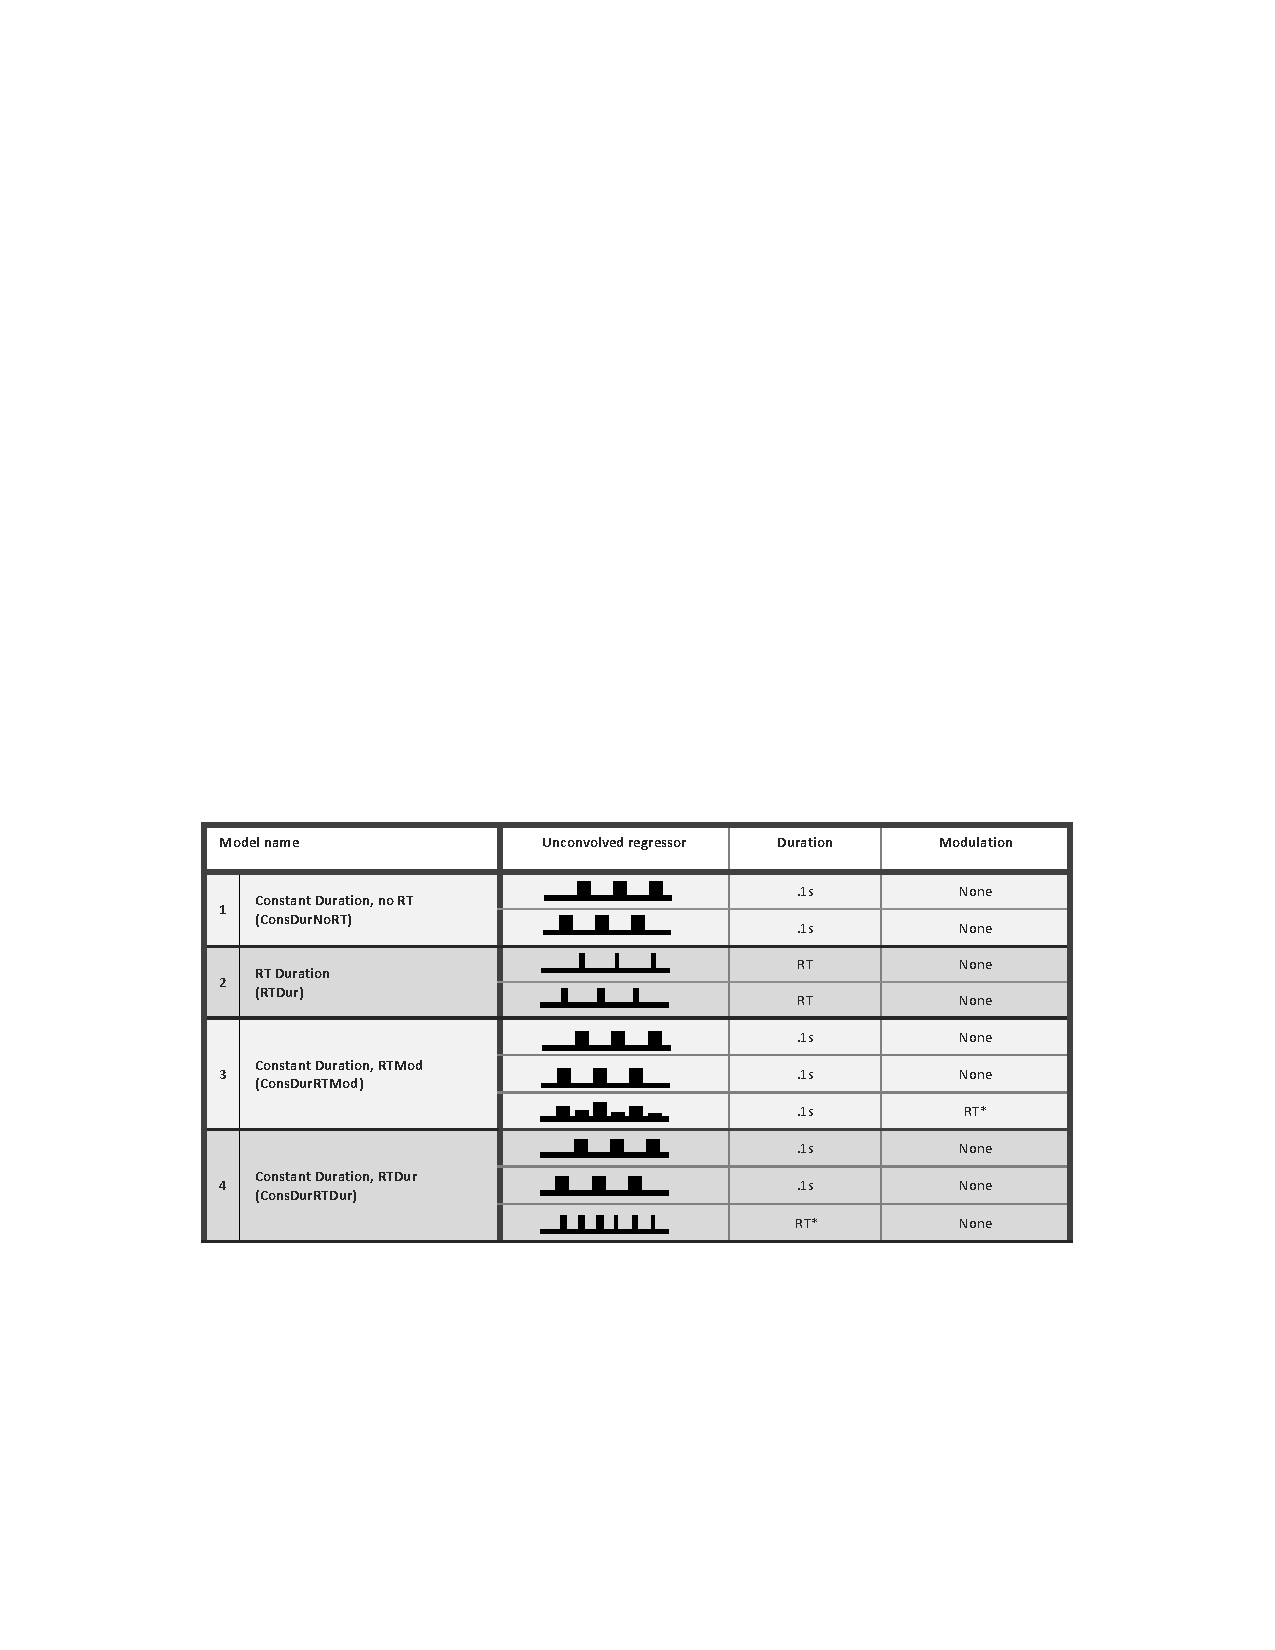
\includegraphics[width=\linewidth]{fig2_model_explainer.pdf}
   \caption{Models assessed in the simulation study.  Models are described by name, unconvolved regressor visualization, duration used for boxcars of unconvolved regressors and definition of the modulation used, when present.  Convolved regressors were used in data generation and modeling.  The first model does not include any response time information, the second model addresses RT through the duration of the regressors and the third and fourth models add an RT regressor to the first model either using an RT modulated regressor (Model 3) or an RT duration regressor (Model 4).  $^*$See Discussion Section for details on why RT is not centered for the RT modulated regressor of Model 3 and why the RT Duration regressor of Model 4 is not orthogonalized.}
  \label{fig:models}
\end{figure}

\citet{grinband_detection_2008} developed a modeling approach to address response times in fMRI data, where boxcar durations for each trial varied by trial response times (labeled as ``RT Duration/RTDur'' in Figure \ref{fig:models}).  This approach will appropriately scale the parameter estimates for regions in which neural activity durations match RT durations, which we will refer to as ``duration scales with RT''. This models an interaction and since constant duration regressors are not included, the model implies each condition has a different linear relationship between BOLD activation and RT, and that BOLD activation is 0 when RT is 0.  One shortcoming of this model is it will not correctly model activation in regions where neural activity duration does \textit{not} scale linearly with RTs.  

To address these issues, we created a generalized model of RT that can identify RT effects separately from the task effect (corrected for RT); the two implementations of this model are shown as ``Constant Duration, RTMod'' (ConsDurRTMod) and ``Constant Duration, RTDur'' (ConsDurRTDur) in Figure \ref{fig:models}.  Each of these models starts with the ConsDurNoRT regressors and adds a single RT regressor.ConsDurRTDur models RTs through duration and ConsDurRTMod models RTs through parametric modulation. In both cases any differences in RTs between conditions will be removed by the RT regressor, leaving the condition difference effects to be interpreted as unconfounded estimates of activation in relation to the experimental manipulation. This model can be extended to a full interaction model by splitting the single RT regressor into two RT regressors, one for each condition.   This will be further described in the Power Analysis results. Notably we have not orthogonalized the RT regressor in ConsDurRTDur or mean centered the RTs in the RT regressor of ConsDurRTMod, which will not have any impact on the estimate of the contrast of interest (condition difference) but may negatively impact the interpretation of other contrasts or introduce RT confounds in group level analyses.  This will be further discussed in the Discussion section.    

Response time data were simulated based on RTs from two different tasks: the Stroop task (based on our data) and reported RT distribution parameters from a two-alternative, forced-choice categorization task from \citet{grinband_detection_2008}.  In each case RTs were generated by sampling from an ex-Gaussian distribution \citep{Ratcliff1976RetrievalPI}; the specified ex-Gaussian parameters led to RTs that were generally longer for the two-alternative, forced-choice categorization task (mean = 1337, sd = 706.5) compared to Stroop (mean = 690, sd = 177.5).  Another difference is the variance relative to the mean is smaller for the Stroop task (coefficient of variation of .528 and .257 for the two-alternative, forced-choice categorization and Stroop tasks, respectively).   Interstimulus intervals (ISIs) were sampled from a Uniform distribution and condition order was randomly presented.  Time-series data where duration scales with RT were generated using the RTDur model and data where duration did not scale with RT were generated using the ConstDurNoRT model. 

For all models the contrast of interest was condition 2 - condition 1 and all simulation-based results correspond to group-level analyses with 100 subjects.  See the Methods for further details.


\subsubsection*{Error rates and power}
 
 We first assessed the false positive rate for each model on each of the simulated data sets for the condition comparison contrast (Figures \ref{fig:type1err_24}, Extended Data Fig. 1). In all cases the ConsDurRTDur model appropriately controlled Type I error but the ConsDurRTMod model failed to control error rates for large RT differences ($>$1s) when the signal duration scales with RT because longer RTs ($>$2s) are not fit as well by an RT modulated regressor.  The modulated regressor assumes the BOLD activation increases linearly with duration, which is an assumption that only holds well for RTs under 2s, which will be explored in detail in the ``RT-based and RT-driven group-level confounds'' section. Due to model assumption violations, ConstDurNoRT had inflated error rates when activation duration did scale with RT, and RTDur had inflated error rates when the signal duration did not  scale with RT.  Thus, the most commonly used model for task fMRI analysis, ConstDurNoRT, suffers from substantial inflation of false positives in the face of RT differences between conditions, because it inaccurately attributes the confounding RT signal to differences in the intensity of the underlying neuronal signal.  Larger Type I error rates observed with the Stroop-based RT reflects a reduced RT standard deviation compared to the forced-choice categorization task, making RT-based differences easier to detect.  Results with a longer ISI (3-6s), are similar (Extended Data Fig. 1).

\begin{figure}[ht!]
  \centering
%   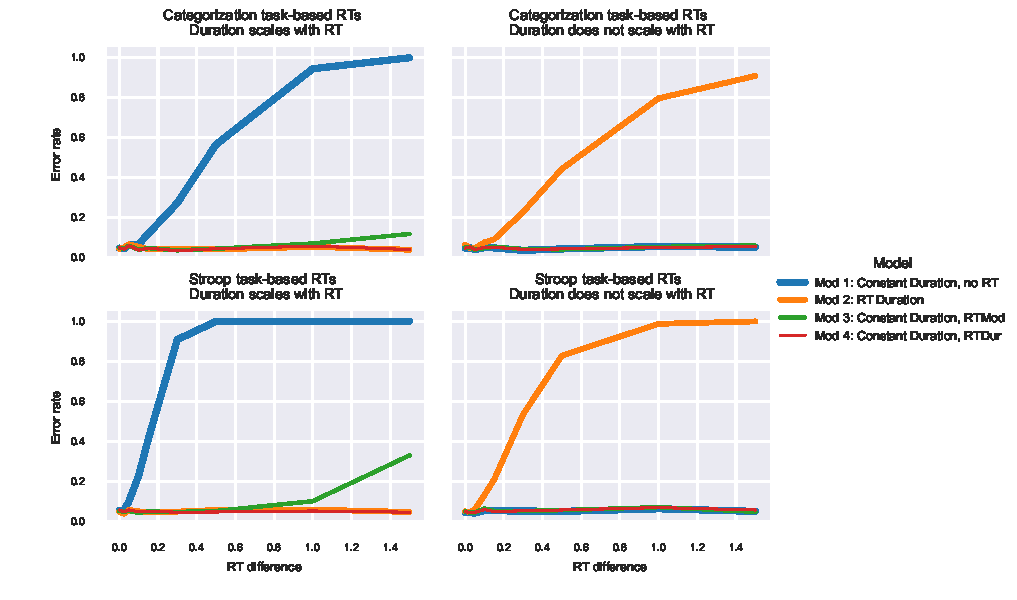
\includegraphics[width=\linewidth]{fig3_type1_err_24_rev.pdf}
   \caption{Type I error as RT difference between conditions increases.  The two-alternative, forced-choice categorization task RT distribution was used in the top panels, while Stroop RT distribution was used in the bottom panels. An ISI between 2-4s was used and the inference of interest was for the 1-sample t-test of the condition difference effect with 100 subjects.  2500 simulations were used to calculate the error rate. Models with error rates larger than .05 are not valid.}
  \label{fig:type1err_24}
\end{figure}


Only models with controlled Type I errors are considered in the power analyses since the inflated error rates indicate bias in the contrast estimates. When signal duration does not scale with RTs, power for ConsDurNoRT (true model) and ConsDurRTDur are compared (right panels, Extended Data Fig. 2) and ConsDurRTMod is only considered if RTs are less than 2s (right panels, Figure \ref{fig:power_rtdiff1}).  In this data setting, the true model, ConsDurNoRT, has maximum power and ConsDurRTDur/ConsDurRTMod have negligable power loss when the RT difference is .1s while ConsDurRTDur has a slight power reduction when the RT differences is .8s (Extended Data Fig. 2). For large RT differences there can be mild collinearity between the RT regressor and the conditions, which explains the power loss.

When signal duration does scale with RTs, power is considered for RTDur (true model) and ConsDurRTDur. The data in this setting follow an interaction effect, so we added a 4 regressor interaction model that combines the regressors from RTDur and ConsDurNoRT, where the contrast of interest is the comparison of the RTDur regressors. When RTs are $<$2s (Figure \ref{fig:power_rtdiff1}), we add a second 4 regressor interaction model using RT modulated regressors, which has been proposed by \citet{carp_conditional_2010, carpRemovingEffectResponse2012, weissman_congruency_2013}. In this setting the RTDur model will have maximal power (orange line, left panels Figures  \ref{fig:power_rtdiff1} and Extended Data Fig. 2).  Interestingly, the ConsDurRTDur model has only a slight power loss when the RT difference is large (red lines, Extended Data Fig. 2) and is negligible for the RT difference of .1s (Figure \ref{fig:power_rtdiff1}).  See Extended Data Fig. 3 for an illustration of how condition differences from ConsDurRTDur can approximate  RTDur differences in this data setting. The 4 regressor interaction models have large losses in power for both RT difference settings (Extended Data Fig. 2  and Figure \ref{fig:power_rtdiff1}). This large power loss is due to variable contrast estimates caused by high collinearity between RT regressors and condition regressors, where the variance inflation factors for the contrast of interest were almost always above the commonly accepted threshold of 5.



\begin{figure}[ht!]
  \centering
%   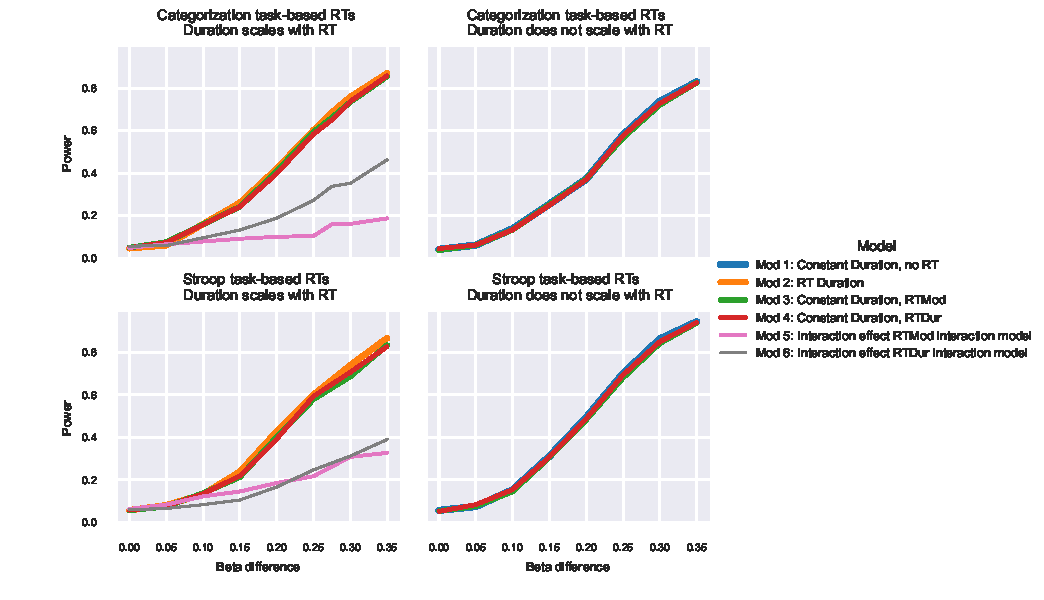
\includegraphics[width=\linewidth]{fig4_power_24_rtdiff_1_all_rev.pdf}
   \caption{Power when the RT difference is 0.1s as the condition difference increases. Only
models that had controlled error rates in Figure 3 are shown. The two-alternative,
forced-choice categorization task RT distribution was used in the top panels (Choice), while
Stroop RT distribution was used in the bottom panels. An ISI between 2-4s was used
and the inference of interest was for the 1-sample t-test of the condition difference
effect with 100 subjects. Model 1, ConsDurNoRT, is the true model for the right column
and model 2, RTDur, is the true model for the left column, so both indicate maximal
power.}
  \label{fig:power_rtdiff1}
\end{figure}




\subsection*{RT-based and RT-driven group-level confounds}

The foregoing analyses, along with the previous work by Grinband, focused on confounding of RT between-trials, which impacts average condition effects.  Here we introduce a new problem of between-\emph{subject} RT confounds.  Within-subject differences in average RT, corresponding to the contrasted conditions, can confound group-level analyses involving group comparisons or associations.  For example, the incongruent versus congruent BOLD contrast estimate may correlate with the differences in average RTs for incongruent and congruent conditions.  This is of particular interest given the increasing focus on analyses of brain-behavior correlations in fMRI literature (e.g., \citet{duboisBuildingScienceIndividual2016}).

The driving factor of correlations between condition differences in brain activation and corresponding differences in RTs is simply due to the relationship between the activation estimate and RT when the data and model assumptions are in conflict. For example, if signal durations scale with RTs and the ConstDurNoRT model is used (duration = 1s), the relationship between the estimated activation, $\hat\beta$, and the true activation, $B$, is approximately $\hat\beta = B \times RT$, for a single trial (left panel, Figure \ref{fig:bold_rt}), where the trend becomes nonlinear after approximately 2s.  As Figure \ref{fig:bold_rt} lays out, this implies the relationship between condition difference estimates and RT differences is given by
\begin{equation}\label{eq:linear}
\hat\beta_2 -\hat\beta_1 = B\times\left(\overline{RT}_2 - \overline{RT}_1\right).
\end{equation}
In the example shown in  Figure \ref{fig:bold_rt}, even though the true condition difference is 0 for all subjects, the average estimated condition difference is nonzero across subjects and also has a linear relationship with the RT difference (right panel, Figure \ref{fig:bold_rt}). As is the case with all linear trends, this relationship does not require a non-zero RT difference on average, but is driven by between-subject RT variability making it a potential confound whenever using ConsDurNoRT.




\begin{figure}[ht!]
  \centering
%   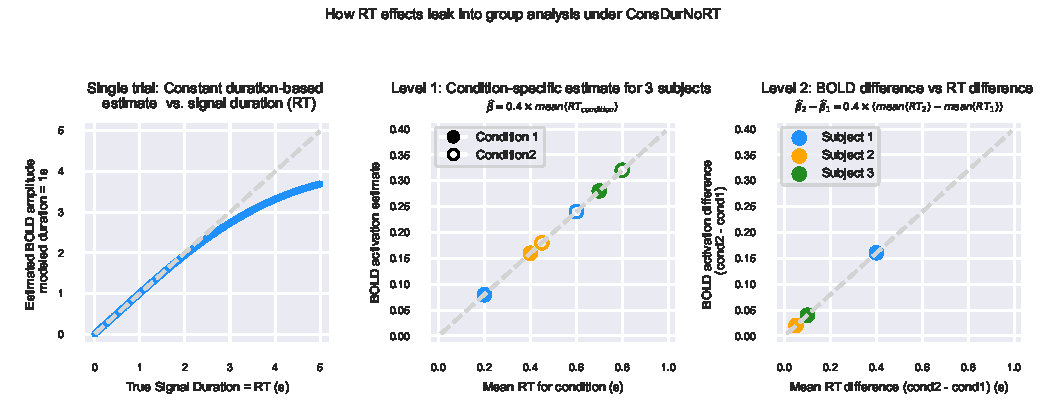
\includegraphics[width=\linewidth]{fig5_bold_fcn_rt_1sdur_only.pdf}
   \caption{The relationship between signal duration and activation estimates and how it can cause RT effects to leak into group analyses when using ConsDurNoRT.  The left panel shows the relationship between the trial duration (RT) and the trial-specific BOLD activation estimate when a constant duration of 1s regressor is assumed and signal duration scales with RT (blue).  The gray dashed line is a line with a slope of 1 and intercept of 0.  The true BOLD activation is 1, but the model estimates the BOLD activation to be $1\times$ RT for RTs $<$ 2s.  After 2s the linear relationship fails to hold, which explains when an RT modulated regressor will begin to fail as the amplitude is no longer a reasonable replacement for duration.  The middle panel is an example of BOLD activation estimates for 3 subjects for 2 conditions when the true activation magnitude is $B=.4$ for both conditions (no condition effect difference) and the RTs are all less than 2s. The BOLD activation estimates are given by $\hat\beta_{cond} = .4 \times mean(RT_{cond})$ for each condition and subject.  The right panel shows that even though the true condition difference is 0, the estimated condition differences are nonzero and vary according to $\hat\beta_2 - \hat\beta_1 = .4 (mean(RT_2) - mean(RT_1))$, and so the contrast estimates are linearly related to the RT difference.}
  \label{fig:bold_rt}
\end{figure}


Simulation results in Figure \ref{fig:rt-cor} show  group RT difference correlations across all models and data types. ConsDurNoRT and ConsDurRTMod   produce correlations between contrast differences and RT differences when signal durations scale with RTs, as does RTDur when signal durations do not scale with RTs. ConsDurRTDur does not induce correlations for either signal type.  Although no true relationship between average subject RT differences and fMRI condition differences exist, the mismatch between model assumptions and data potentially introduce a group-level model RT confound.  We did not introduce a specific between-subject variance in the RT difference, implying the between-subject variance may be underestimated, but we did not want to artificially inflate the effect.  Even so, it is within the ballpark of the expected true correlations between brain and behavior measures \citep{marekReproducibleBrainwideAssociation2022}.  


In the previous example, the linear relationship at the group level is, $B$, the common activation for both conditions and all subjects, but if activation differs between conditions or across subjects the confound will be more complex and can even introduce new artifactual associations into group analyses.  To illustrate how false associations can be introduced, relax the assumption that $B$ is the same across subjects, but preserve the assumption that $B$ is the same for both conditions.  For example, assume time spent outdoors ($TO$) is equally related to both conditions through the relationship, 
\begin{equation}\label{eq:to}
B=\gamma_0 + \gamma_1 TO + \epsilon,
\end{equation}
noting $TO$ is not related to the true difference in activation between conditions or RTs. If the signal durations scale with RTs and ConsDurNoRT is used to estimate condition differences, both an artifactual  RT difference effect and an artifactual RT difference by $TO$ interaction are introduced to group-level data.  This can be seen by combining equations \ref{eq:linear} and \ref{eq:to}:

\begin{align}
  \hat\beta_1 - \hat\beta_2 &= (\gamma_0 + \gamma_1 TO)\times \left(\overline{RT}_1 - \overline{RT}_2\right) \\ \nonumber
  &= \gamma_0\left(\overline{RT}_1 - \overline{RT}_2\right) + \gamma_1 TO \left(\overline{RT}_1 - \overline{RT}_2\right).
\end{align}

Due to the interaction effect with $TO$ and the nonlinear impact of RT on the BOLD signal when RTs$>$2s, adding RT difference as a confound regressor to the group model will not remedy these issues and should be avoided as it may inflate the significance of the false association with $TO$.  The relationship between RT and potential variables of interest will be more complex if the RT difference is correlated with that variable or if the true activation difference and the variable of interest are correlated. This cannot be repaired within group-level analyses, but only by replacing  first-level analyses with ConsDurRTDur. This is unsettling news for those using fMRI activation databases, since the ConsDurNoRT model is typically used to generate activation estimates and, as the next section underlines, the presence of RT effects is widespread.

\begin{figure}[ht!]
  \centering
%   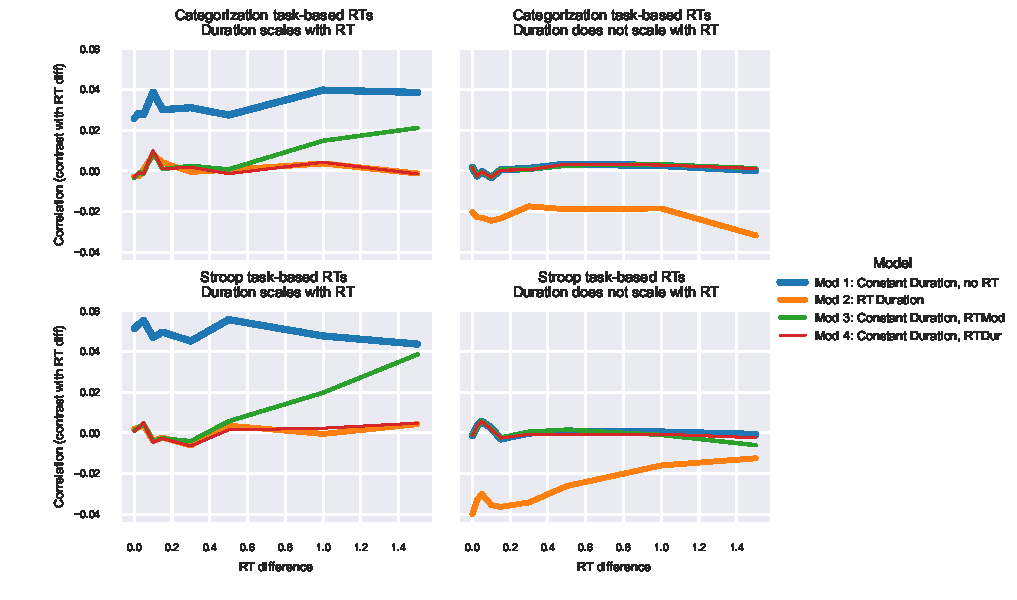
\includegraphics[width=\linewidth]{fig6_cor_with_rt_rev.pdf}
   \caption{Correlation between the contrast difference and difference in average condition RT across subjects as a function of the average difference in RT between conditions.  Since the correlation is driven by between-subject variability in the \emph{difference} in RT, there is no requirement that RTs differ between tasks and the correlation is constant regardless of the RT difference. In the case of ConsDurRTMod (green line, left panels) the correlation increases when the duration scales with RT for higher RT differences due to increasing model misfit as RTs increase (see Figure \ref{fig:bold_rt}).}
  \label{fig:rt-cor}
\end{figure}


\subsection*{Widespread RT activation is not specific to task, revisited}

Our real data analyses were modeled to included separate condition regressors and a single RT duration regressor, following ConsDurRTDur.  A total of 7 tasks, with sample sizes ranging from 86 to 94, were analyzed. The cognitive processes involved in these tasks include attention, temporal discounting, proactive control, reactive control, response inhibition, resisting distraction, and set shifting.  Brief descriptions are given in Supplemental Table 1 and more detailed summaries are provided in the Methods section (``Details about tasks involved in real data analysis'') and Supplementary Materials.  Comparatively, \citet{yarkoni_bold_2009} used tasks including  3-back, decision making, emotion ratings and memory in sample sizes of 50, 102, 26, 35 and 39. Our seven tasks emphasize cognitive control to a greater extent and emotional processing and working memory to a lesser extent, compared to \citet{yarkoni_bold_2009}.   The focus here is on average RT-related effects across subjects.  This effect estimate will be slightly diminished from a full RT effect, since it is adjusted for condition difference. The interpretation is the average within-condition RT effect.  Figure \ref{fig:conj} shows voxels where the average RT-duration effects were significant across all 7 tasks.  Our maps are consistent with \citet{yarkoni_bold_2009}, but with a more spatially widespread effects, which may reflect that our sample sizes were larger. In particular, the present comparison demonstrated substantially more signal in the lateral superior parietal cortex.

To illustrate how the RT-based network overlaps with and does not overlap with condition difference effects, Extended Data Fig. 4 illustrates group average results where only the RT effect was statistically significant (yellow), where only the condition comparison was significant (blue) and the overlap (green) for a single contrast from each task where ConsDurRTDur was used. Using the Stroop task as an example, the expected dMFC activation for incongruent versus congruent is present even though RT was included in the time series model.  Although there is often overlap in the activation for the RT effect and the condition comparison, there are regions where only the condition comparison is active.




\begin{figure}[ht!]
  \centering
%   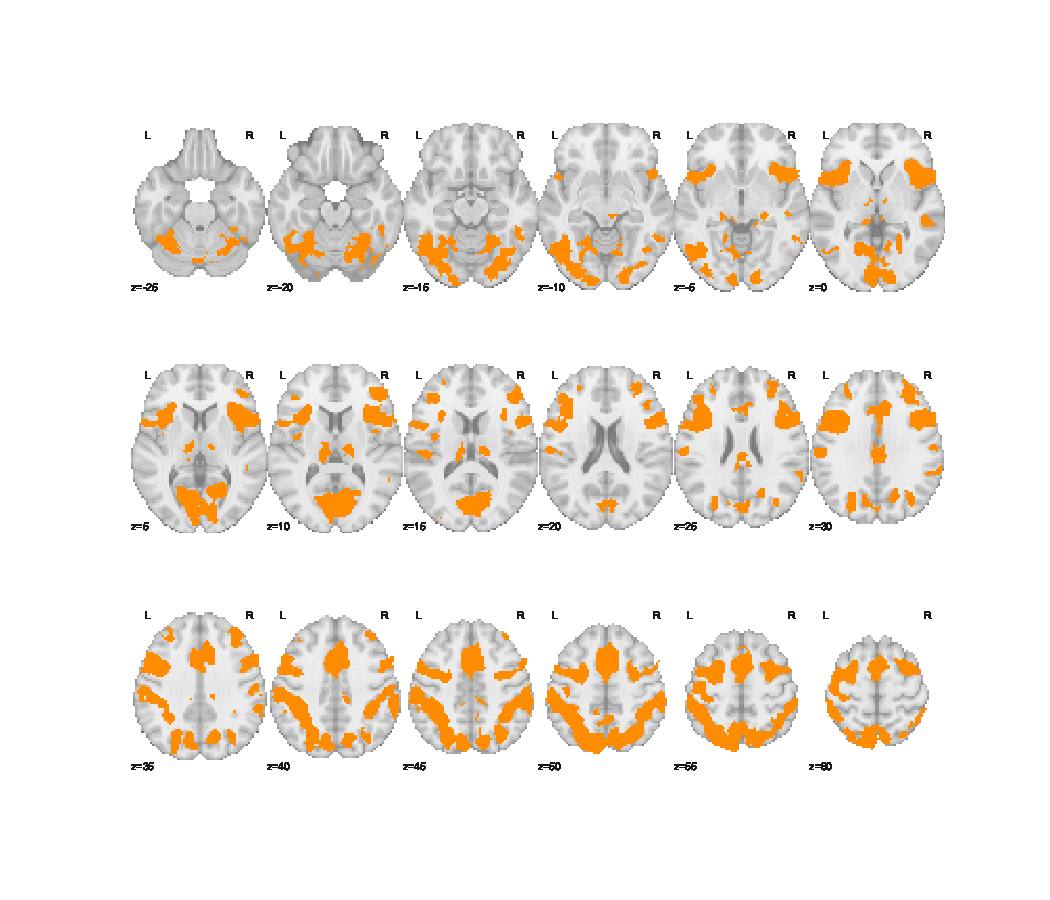
\includegraphics[width=\linewidth]{fig7_conjunction_avg_rt_effect_across_7tasks_3row_plot.pdf}
   \caption{Conjunction of the average, within-condition RT effect across ANT, DDT, DPX, motor selective stop, stop signal, stroop, and CTS.  On average, each analysis included around 91 subjects and maps were corrected for multiple comparisons using a TFCE p-value thresholded at 0.05 using 5000 permutations.}
  \label{fig:conj}
\end{figure}




\section*{Discussion}

The problem of potential response time confounds for fMRI activation estimates has been discussed for more than a decade, with little resulting change in how the community approaches analyses and interpretations of fMRI contrasts.  There are three takeaways from the present work.  First, we propose a modeling approach that can adapt to fit data whether or not activation durations scale with RTs.  Importantly this model does not remove the ability to also study RT-specific effects, if they are of interest.  Second, this work highlights an important problem that has not been discussed previously: 
the presence of a between-subject confound of the average RT differences and the potential to introduce artificial associations with variables of interest at the group level.  Finally, we replicate the work of \citet{yarkoni_bold_2009} showing widespread RT-related effects that are not task specific.

This work presents a model that can adapt to whether or not signal durations scale with RTs, with limited performance loss. By adding an RT duration regressor to the most commonly used model that only contains condition-specific regressors, ConsDurRTDur removes RT-driven type I errors in average condition comparison effects with a slight reduction in power when the signal durations do not scale with RTs and the RT difference is large.  The commonly used ConstDurNoRT model assumes signal durations do not scale with RTs and the RTDur model assumes  signal durations must scale with RTs, and both models fail to control error rates when these model assumptions are violated (Figure \ref{fig:type1err_24}).  Interestingly, when RTDur is correct (interaction effect), only a slight power loss results when using ConsDurRTDur, while a 4 regressor interaction model has a large power loss due to collinearity in the  model. This implies the ConsDurRTDur model can still be useful in detecting condition differences that arise through interactions that follow the RTDur model, although for regions with a hypothesized interaction, RTDur should be used to maximize power.    


We have also uncovered that subject-specific differences in average RT represent an important group-level confound.  This confound is only present when using ConsDurNoRT, RTDur or ConsDurRTMod when RT differences are large, whereas the ConsDurRTDur model produces condition difference effects that are free of this confound.  Notably, the average difference in RT across subjects does not necessarily impact correlation strength, since correlations are driven by variability, in this case variability in RT differences across subjects.   Thus, even if the average RT difference is 0, the first-level models should follow ConsDurRTDur.  We have also shown that when signal durations scale with RTs and ConsDurNoRT is used, other false associations can be introduced at the group level. When there is a common association between a variable of interest (e.g., time spent outdoors) and each condition, separately, but no association of this variable with the true condition difference, the ConsDurNoRT condition difference estimates can have false associations with this variable. This is a concerning result for users of neuroimaging databases of condition difference estimates, since ConsDurNoRT is typically used.


Last, our updated RT-effect conjunction analysis across 7 tasks tapping into different mental processes show widespread shared activation in the so-called ``task-positive'' network, replicating the previous results of \citet{yarkoni_bold_2009}. This highlights the generality of the RT effect across tasks, and motivates the need to model these effects across all tasks.  

%\subsection*{Paradox: RT is the effect of interest in fMRI studies}

There may be resistance to adding an RT duration regressor to convert ConsDurNoRT to ConsDurRTDur, since RT is the measure of interest in behavioral studies and removing RT effects from condition differences might be argued to be ``throwing the baby out with the bathwater''.  This argument is paradoxical because if RT is the effect of interest, why would it be ignored in the fMRI model?  ConsDurNoRT can find significant results for any of the scenarios in Figure \ref{fig:underlying-theory}, and when the data follow ``RT effect only'' the results likely reflect false positives as shown in our Type I error simulation results.  The ConsDurRTDur model is flexible, fitting signal when durations do or do not scale with RT. ConsDurRTDur can fit data that follow any of the scenarios in Figure \ref{fig:underlying-theory}, without resulting in false positives for the ``RT effect only'' scenario and with a slight power loss only when there is an interaction between condition and RTs.  The flexibility of ConsDurRTDur means it does not align with a specific behavioral model. If a specific link between the underlying cognitive theory and the fMRI model is of interest, this requires motivating why that theory would hold and for which specific regions of interest.  Then, for those regions of interest the fMRI model that aligns with the underlying theoretical model should be used.  For example, if theory supports that a region would elicit brain activation where neuronal duration scales with RT, then RTDur will have the highest power and should be used for that region rather than ConsDurRTDur.  That said, RTDur is not likely appropriate in a whole brain analysis since it is not designed for regions where the signal duration does not scale with RTs as stated in \cite{grinband_detection_2008} and illustrated by elevated Type I errors in our simulations. 




\begin{figure}[ht!]
  \centering
%   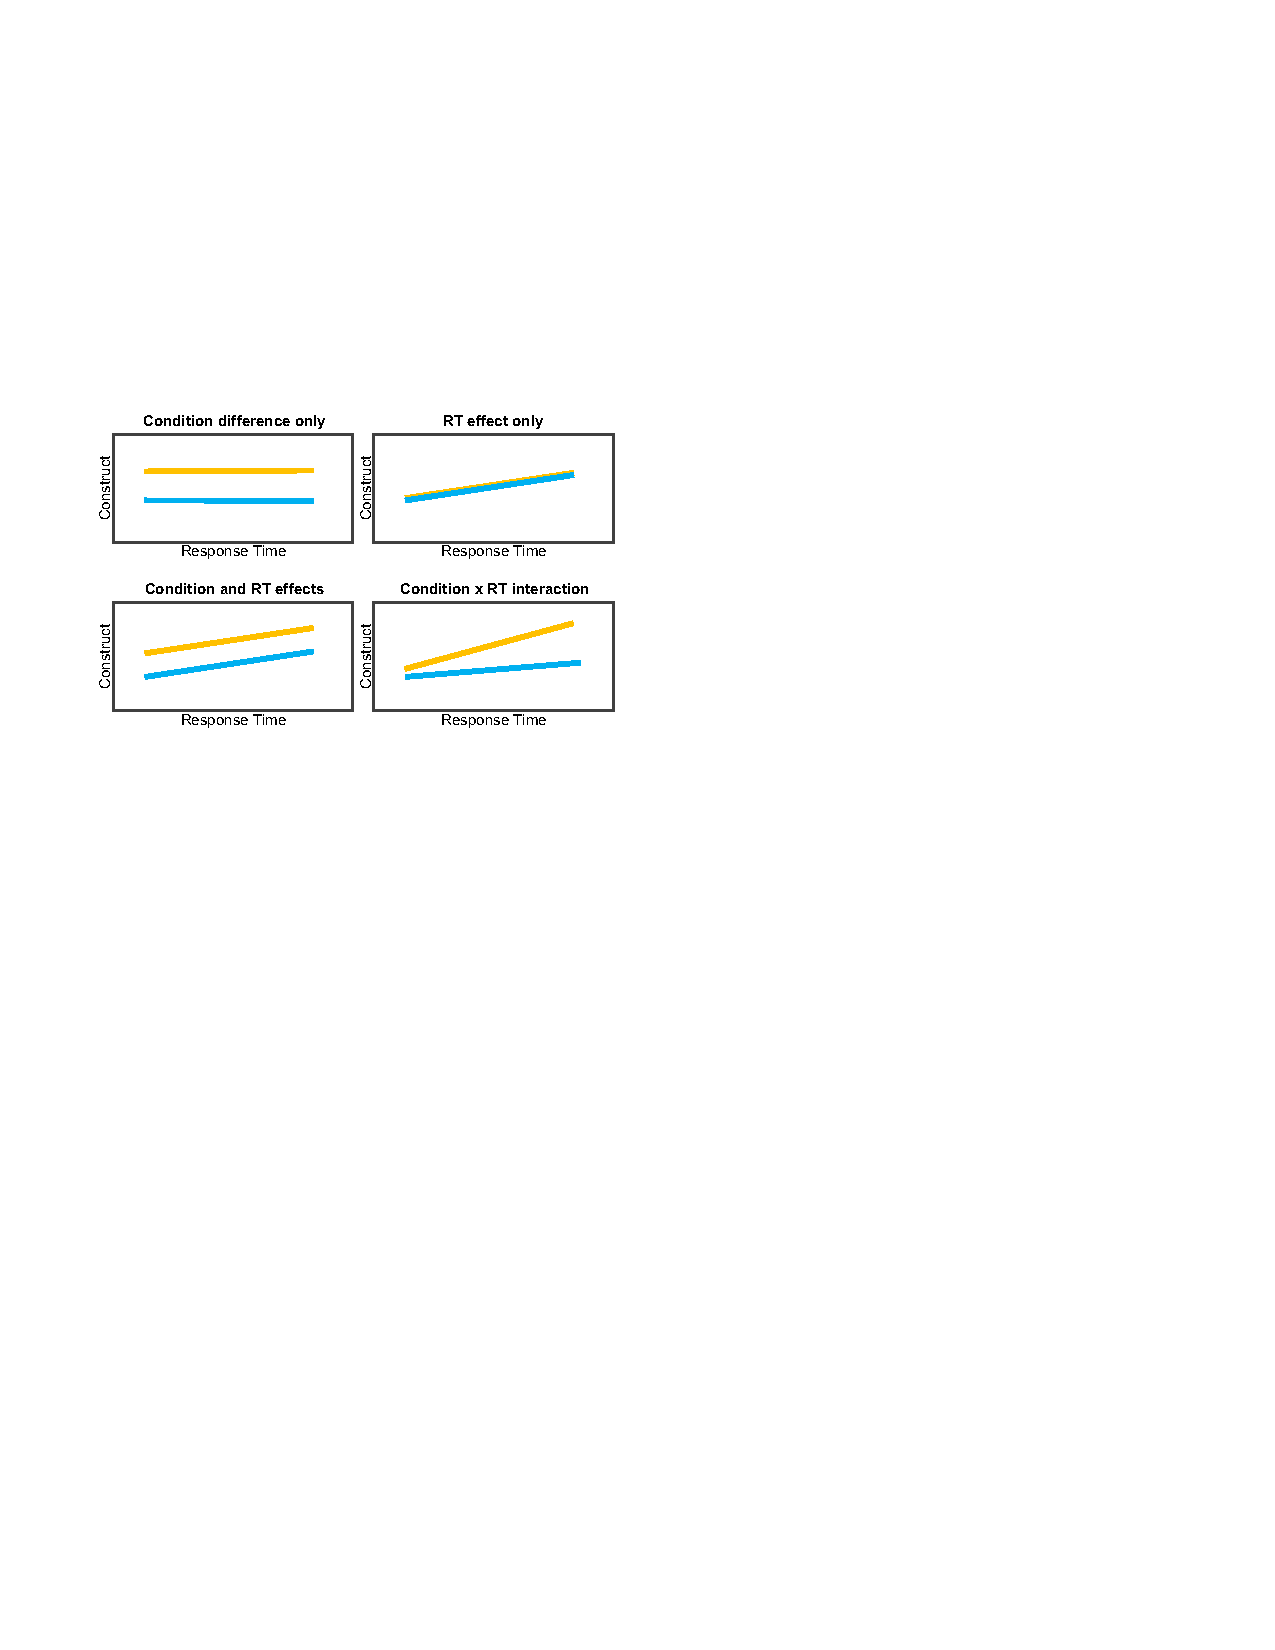
\includegraphics[width=\linewidth]{fig8_underlying_theory.pdf}
    \caption{Examples of the underlying relationship between a behavioral construct and RTs.}
  \label{fig:underlying-theory}
\end{figure}


%\subsection*{Contrast interpretation from ConsDurRTDur and ConsDurRTMod}
Both ConsDurRTMod and ConsDurRTDur assume that  mean task activation differs for each condition while the BOLD/RT relationship is the same for both conditions, analogous to a regression model that models two parallel lines corresponding to two conditions.  Condition differences, when both conditions involve RTs, will be the same regardless of the value of RT.  Conversely, a contrast of a condition involving RTs vs baseline, or a comparisons of conditions where only some of the conditions involve RTs, will vary by RT.  Any estimate of these contrasts will reference a specific RT.  For example, the contrast interpretation for conditions involving RTs versus baseline correspond to the activation magnitude for a trial with an RT of 0, which is illustrated in the middle panel of Extended Data Fig. 3  where the condition 1 (orange) has a negative task versus baseline effect while the condition 2 (blue line) has a small positive effect in the ConsDurRTDur model.   Extended Data Table 1 illustrates examples of contrast interpretations using the Stroop task.  It may be tempting to use orthogonalization so the interpretations do not correspond to an RT of 0, but the following section outlines the limitations of this idea.



%\subsection*{Orthogonalization of regressors}

A common misunderstanding is that collinearity between regressors is problematic and orthogonalization should be used to remove collinearity or to change parameter interpretation.  Orthogonalization is almost never necessary and is often applied incorrectly, leading to confusion in interpretation \citep{mumford:poline:poldrack:2015}.  In the case of ConsDurRTDur and ConsDurRTMod, orthogonalization of the RT regressor can change the interpretations of contrasts so they do not correspond to an RT of 0. Extended Data Table 2 describes various orthogonalization strategies for ConsDurRTDur and ConsDurRTMod and explains how contrast interpretation is impacted and whether orthogonalization is acceptable.  For ConsDurRTDur, orthogonalization of the RT regressor with respect to each condition (row 1) is problematic because condition differences are no longer adjusted for RTs.  Rows 2 and 3 show how ConsDurRTDur and ConsDurRTMod can orthogonalize the RT regressor with respect to all RT-based trials, but this introduces a between-subject RT confound, which is not acceptable.  The last row describes a way to center RTs in ConsDurRTMod that avoids the between-subject RT confound, where all contrasts that previously corresponded to an RT of 0 now correspond to some specific RT, $C$.  This practice is questionable since, if the RT relationship is positive, selecting a larger value for $C$ will inflate the contrast estimate.


Importantly, issues with the contrast interpretations presented in Extended Data Table 1 only arise in analyses of single group means while group comparisons and associations with other variables are not impacted by the reference RT value for a contrast, as long as it is constant across subjects.




 
%\subsection*{Limitations of this work}
The present work provides a modeling framework for moving forward, but it is likely that as researchers start thinking about response times more carefully, the model will need to be further adapted. For example, it is challenging to simply apply the ConsDurRTDur model to the stop signal task since the overt response process is unobservable on some trials (i.e. successful stop trials), and the stop process is generally estimated at a block- or session-level so is unobservable on all individual trials. It is unclear how the absence of this time in the models impacts results. Although it is beyond the scope of this work to find a solution to this problem, this is a future direction we will explore.


This work consists of real data analyses as well as simulated data analyses.  Simulations are required in cases where we need to know the ground truth and link the theoretical problems with how these problems might surface in real data analyses (e.g., how strong the results are and whether they persist at the group level). As such, the simulations require specifying a large number of parameters including the RT distribution for each condition, effect size for each condition, stimulus length, ISI,  within-subject variance and between-subject variance.  Our simulation parameter choices are described in the Methods section and we feel generated realistic simulated data as the results are consistent with similar studies  \citep{yarkoni_bold_2009, brown_medial_2011, grinband_dorsal_2011}. 

\section*{Methods}
This fMRI study described below (``Real Data Analysis'') was approved by the Stanford University Institutional Review Board (approval number: 39322) and complies with all ethical regulations.
\subsection*{Models considered}

\subsubsection*{Data generation and modeling} 


The interstimulus interval (ISI) was sampled from a Uniform distribution and RT was sampled from an ex-Gaussian distribution.  For RT, a subject specific mean, $m_s$, was obtained by sampling an ex-Gaussian with parameters $\mu_{rt}$, $\sigma_{rt}$ and $1/\lambda_{rt}$.  The mean of an ex-Gaussian distribution is the sum of $\mu$ and $1/\lambda$ and in our Stroop data the within-subject estimates of $\mu$ were approximately 76\% of the mean.  Using this information the $\mu$ and $1/\lambda$ parameters for  fast RTs that differed by $\Delta RT$ were defined by $\mu_{fast} = .76m_s - .76 \Delta RT/2$ and $1/\lambda_{fast} = .24 m_s -.24 \Delta RT/2$, respectively.  The slow RTs were obtained similarly but used addition.  This preserved the desired mean RT difference and also allowed the variance to change with the mean RT, since $\lambda$ contributes to the variance as well.  Values of $\mu_{rt}$, $\sigma_{rt}$ and $\lambda_{rt}$ were based on our Stroop data and the two-alternative, forced-choice categorization task in \citet{grinband_detection_2008}.  In both cases distributions were fit to subject-specific data and then parameters were averaged over subjects.  The two-alternative, forced-choice categorization task RT distribution was defined by a Gamma distribution with shape parameter = 1.7, beta = 0.49.  Sampling from this distribution and fitting an ex-Gaussian to that sample resulted in ex-Gaussian parameters of $\mu_{rt} = 638$, $\sigma_{rt} = 103$, and $1/\lambda_{rt} = 699$ (mean = 1337, sd = 706.5). The Stroop data had faster RTs with less variability, with ex-Gaussian parameters of  $\mu_{rt} =530$, $\sigma_{rt} = 77$, and $1/\lambda_{rt} = 160$ (mean = 690, sd = 177.5).  The distribution functions from the Scipy module (v 1.9.1)  of Python (v 3.9.7) were used to simulate and estimate the distribution parameters. Trial order was  random.
 


Simulated data where signal duration scaled with RT were created with the convolved RT duration regressors (RTDur) and data where signal duration did not scale with RT used the constant duration regressors (ConsDurNoRT).  The BOLD activation sizes, $\beta_{i,j}$, for the $i^{th}$ subject for $j^{th}$ condition ($j$ = 1,2)  were  sampled from a Gaussian distribution, $N(\beta_j, \sigma_b^2)$,  where $\beta_j$ is the true activation magnitude and $\sigma^2_b$ is the between-subject variance.  The time-series data for the $i^{th}$ subject, of length $T$, was created according to 
\begin{equation} \label{eq:timeseries}
   \vb{Y_i} = \vb{X}_{1}\beta_{i, 1}  +  \vb{X}_{2}\beta_{i, 2} + \epsilon, \hspace{.1in} \epsilon \sim N(0, \sigma^2_w), 
\end{equation}
where $\vb{X}_{1}$ and $\vb{X}_{2}$  are either the Model 1 or 2 regressors $(T\times 1)$  and $\sigma^2_w$ is the within-subject variance.  


In an effort to choose realistic values for $\beta_1$, $\beta_2$, $\sigma^2_w$ and $\sigma^2_b$, we considered the first-level effect size (converting the true $\beta_i$ to a  correlation), second level effect size for a 1-sample t-test (Cohen's D) as well as the ratio of the total mixed effects variance to the within-subject variance.  Following the definitions of parameters as given in the model above, the total mixed effects variance for a first-level contrast of parameter estimates is
\begin{equation} \label{eq:mfxvar}
 \sigma^2_{mfx} =  \vb{c}(\vb{X}'\vb{X})^{-1}\vb{c}'\sigma^2_{w} +\vb{c}\vb{c}'\sigma^2_b,
\end{equation}
where $\vb{X}$ and $\vb{c}$ are the first-level design matrix (based on models in Figure \ref{fig:models}) and contrast of interest \citep{mumford_modeling_2006}.  The contrast of interest for each model corresponded to condition 2 $>$ condition 1 ($\vb{c}=[-1,1]$ for the 2 regressor models and $\vb{c}=[-1,1, 0]$ for the three regressor model).  The ratio of total standard deviation (SD) to within-subject SD is defined by
\begin{equation}\label{eq:sd_ratio}
\frac{SD_{total}}{SD_{within}} = \frac{\sqrt{\vb{c}(\vb{X}'\vb{X})^{-1}\vb{c}'\sigma^2_{w} + cc'\sigma^2_b}} {\sqrt{\vb{c}(\vb{X}'\vb{X})^{-1}\vb{c}'\sigma^2_{w}}},
\end{equation}

Our within-subject effect size for condition versus baseline was between 0.07-0.08 (correlation), ratio of total variance to within-subject variance, $\frac{SD_{total}}{SD_{within}}$,  ranged between 2-3 and the Cohen's D for the average of task versus baseline across subjects was approximately 0.85.

Each run contained 40 trials of each condition and a time resolution (TR) of 1s.  Time course length varied, as it was set to extend 50s past the last stimulus offset.  Group analyses included 100 subjects.  A total of 1000 data sets were simulated to calculate power and error rates. 


Regressors were constructed by convolving boxcar functions with a Double Gamma hemodynamic response function (HRF) using the \verb+spm+ HRF within the \verb+compute_regressor+ function from the Nilearn (v 0.9.1) module in Python (v 3.9.7).  

Least squares regression was used to estimate the models described in Figure \ref{fig:models} at the first-level including a set of cosine basis functions (0.1 Hz cutoff) for high-pass filtering generated with the \verb+cosine_drift+ function from Nilearn (v 0.9.1) in Python (v 3.9.7).  At the group level, 1-sample t-tests were used to assess type I error and power.  A correlation of the average difference in RT between conditions and the fMRI contrast (condition 2 vs condition 1) was estimated for each group analysis.  

Since RT and ISI values are random, the contribution of the design matrix, $X$, to the overall variance varies between samples (Equation \ref{eq:mfxvar}) and the true effect size was variable.  Therefore, to calculate the first-level true effect size 100 data sets were simulated and the partial correlation coefficient for one condition, controlling for the other condition and cosine basis set, was estimated and then averaged over the 100 data sets to serve as the true within-subject effect. The variance ratio, $SD_{total}/SD_{within}$ , was estimated by simulating 100 design matrices.  Cohen's D estimates were based on 5000 simulated within-subject model estimates for the task versus baseline contrast.

\subsubsection*{Real data analysis}

Informed consent was obtained from all human participants and participants were paid \$20 per hour for their participation in the MRI sessions and \$10 per hour for participation in practice and setup time. None of the analyses were preregistered. No statistical methods were used to determine sample sizes, although our sample is about twice as large as the data sets involved in a similar analysis in \citet{yarkoni_bold_2009}.  

Prospective participants for the study were recruited from the Stanford campus and surrounding San Francisco Bay Area using several methods including paper flyers, the Stanford Sona recruitment system, local newspapers ads, the Poldrack Lab website, online resources such as Craigslist, and through email listservs maintained by the Stanford Psychology Department. All recruited participants met the following criteria: have a minimum 8th grade education, speak English fluently, right-handed, have normal or corrected to normal vision and no color-blindness, are between 18-40 years old, have no current diabetes diagnosis, have no history of head trauma with loss of consciousness, cerebrovascular accident, seizures, neurosurgical intervention, stroke, or brain tumor, have no current major psychiatric disorders (including schizophrenia and bipolar disorder) or substance dependence, are not currently using any medication for psychiatric reasons, are not currently pregnant, and have no other contraindications to MRI.

A total of 113 participants were recruited for the study. 3 participants were dropped during their first scan session due to complications in the scanner leaving 110 participants.  The mean age was 23.8 years (sd = 5.5) and 71 participants were female.  The sample had the following demographic distribution: 40\% White, 36\% Asian, 10\% More than one race, 8\% Black or African American, 3\% Unknown, 2\% Native Hawaiian or Pacific Islander, and 1\% American Indian or Alaska Native. The fMRI tasks included: Stroop \citep{stroop_1935}, Attention Network Test (ANT, \citet{fanTestingEfficiencyIndependence2002}), Dot Pattern Expectancy task (DPX, \citet{macdonald2005}), Delayed-Discounting task (DDT, \citet{kirby2009}), cued task-switching task (CTS, \citet{logan2003}), stop signal task \citep{logan1984} and a motor selective stop signal task \citep{dejong1995}.  Brief summaries are provided in  Supplemental Table 1 and more detailed descriptions are provided in the Supplementary materials (``Details about tasks involved in real data analysis'').  Data were acquired using single-echo multi-band EPI using a GE Discovery MR750 3T scanner and a Nova medical 32-channel head coil. The following parameters were used for data acquisition: TR = 680ms, multiband factor = 8, echo time = 30 ms, flip angle = 53 degrees, field of view = 220 mm , 2.2 $\times$ 2.2 $\times$ 2.2 isotropic voxels with 64 slices.

Raw task behavior during scans were collected using Experiment Factory (\url{https://www.expfactory.org/}; \cite{sochat_2016}) running on Macbook laptops.  The raw data can be found at \url{ https://openneuro.org/datasets/ds004636/} and a Data Descriptor paper is available at \citet{dd_preprint}.



Data were preprocessed in Python using fmriprep 20.2.0 \citep{esteban2019}.  First, a reference volume and its skull-stripped version were generated using a custom methodology of fMRIPrep. A B0-nonuniformity map (or fieldmap) was directly measured with an MRI scheme designed with that purpose (typically, a spiral pulse sequence). The fieldmap was then co-registered to the target EPI (echo-planar imaging) reference run and converted to a displacements field map (amenable to registration tools such as ANTs) with FSL’s fugue and other SDCflows tools. Based on the estimated susceptibility distortion, a corrected EPI (echo-planar imaging) reference was calculated for a more accurate co-registration with the anatomical reference. The BOLD reference was then co-registered to the T1w reference using bbregister (FreeSurfer) which implements boundary-based registration \citep{greve2009}. Co-registration was configured with six degrees of freedom. Head-motion parameters with respect to the BOLD reference (transformation matrices, and six corresponding rotation and translation parameters) are estimated before any spatiotemporal filtering using mcflirt (FSL 5.0.9, \citet{jenkinson2002}). BOLD runs were slice-time corrected using 3dTshift from AFNI 20160207 (\citet{cox1997}, \verb+RRID:SCR_005927+). The BOLD time-series (including slice-timing correction when applied) were resampled onto their original, native space by applying a single, composite transform to correct for head-motion and susceptibility distortions. These resampled BOLD time-series will be referred to as preprocessed BOLD in original space, or just preprocessed BOLD. The BOLD time-series were resampled into standard space, generating a preprocessed BOLD run in MNI152NLin2009cAsym space. First, a reference volume and its skull-stripped version were generated using a custom methodology of fMRIPrep. Automatic removal of motion artifacts using independent component analysis (ICA-AROMA, \citet{pruim2015}) was performed on the preprocessed BOLD on MNI space time-series after removal of non-steady state volumes and spatial smoothing with an isotropic, Gaussian kernel of 6mm FWHM (full-width half-maximum). Corresponding “non-aggresively” denoised runs were produced after such smoothing.  These data were used in our time-series analysis models.


Data were analyzed using \verb+FirstLevelModel+ from nilearn in Python (version 3.9.7) \citep{abrahamMachineLearningNeuroimaging2014}.  A double gamma HRF was used for convolution and an AR(1) model addressed temporal auto correlation.  Specifically the \verb+spm+ HRF setting was used, which follows the HRF from the SPM software package with a 6s delay of response (relative to onset), a 16s delay of undershoot (relative to onset), 1s dispersion of response, 1s dispersion of undershoot, a ratio of response to undershoot of 6 and a 32s long kernel.  Regressors were included for each condition, versus baseline, as well as a single RT modulated regressor, similar to the simulation analysis model ConsDurRT.  The RT modulated regressor included the uncentered RT values.  The contrast of the RT modulated regressor was the contrast of interest in our models and represents the average relationship between BOLD activation and RT within condition, since condition specific regressors were also included.  Nuisance regressors in the time-series analysis included the following from the fmriprep output: cosine basis functions (corresponding to a highpass filter cutoff of 128s) and the average time courses for the CSF and WM as estimated by fmriprep. 

Subjects were excluded within-task for the following general reasons: missing 1 or more files required to analyze the data, having more than 20\% high motion time points (measured by Framewise Displacement $>$ .5 or SD of DVARS $>$ 1.2), having more than 45\% missing responses, a subjective poor performance rating assessing high choice and/or omission error rates in at least one condition of the task, and when subjects omitted most of their responses towards the end of the task scan.  Specific exclusion for the stop signal tasks are less than 25\% successes for stop trials or more than a 75\% successful stop rate.  For the Delay-Discounting tasks, subjects were excluded if they made the same choice on all trials.  Last, if there were exclusions on more than half the tasks for a subject, that subject was completely excluded. Exclusions for each task are reported in the supplemental materials (``Exclusion information by task for real data analysis''). 

Group models were estimated using Randomise \citep{smith2009} and included either a single column of 1s (group mean) or a column of 1s along with the difference in mean RTs. Statistics maps were thresholded, controlling for family-wise error rate, using the Randomise TFCE statistic below 0.05, based on 5000 permutations.  Two sided hypotheses were studied using an F-contrast.  A conjunction map was constructed by taking the overlap of the thresholded, binarized map for each of the 7 tasks \citep{nichols_valid_2005}.


\subsection*{Data availability}
The conjunction map (Figure \ref{fig:conj}) and separate RT-based activation maps for each task used to generate the conjunction map are available in the form of 1-pvalue maps at \url{https://neurovault.org/collections/13656/}. Full, raw fMRI data sets are available on OpenNeuro at \url{ https://openneuro.org/datasets/ds004636/}.

\subsection*{Code availability}
The code for all analyses are shared at \url{https://doi.org/10.5281/zenodo.8083510} (simulations) and \url{https://doi.org/10.5281/zenodo.8083518} (real data analysis). 

\subsection*{Acknowledgements}
This work was supported by the National Institutes of Health (NIH) Science of Behavior Change Common Fund Program through an award administered by the National
Institute for Drug Abuse (NIDA) (UH2DA041713; PIs: Marsch, LA \& Poldrack, RA).  The funders had no role in study design, data collection and analysis, decision to publish or preparation of the manuscript.

We would also like to thank Daniel Weissman for discussions that helped in the writing of this manuscript.



\subsection*{Author contributions}
Jeanette Mumford developed the project, wrote all simulation code and much of the real data analysis code, helped with quality assessments of the real data and did most of the writing.  Patrick Bissett helped with model construction, interpretation, data collection and writing of the manuscript.  Henry Jones, Sunjae Shim and Jaime Rios all helped in the collection, preprocessing, quality assessment and analysis of the real fMRI data.  Russell Poldrack helped with model development, interpretation and writing of the manuscript.

\subsection*{Ethics declarations}

The authors declare no competing interests.


%\clearpage % ensure all floats are processed
%\processdelayedfloats
%\clearpage
%\bibliographystyle{elsarticle-harv}
%\bibliography{rt_group}



%% BioMed_Central_Bib_Style_v1.01

\clearpage

\processdelayedfloats

\clearpage

\begin{thebibliography}{41}

% BibTex style file: bmc-mathphys.bst (version 2.1), 2014-07-24
\ifx \bisbn   \undefined \def \bisbn  #1{ISBN #1}\fi
\ifx \binits  \undefined \def \binits#1{#1}\fi
\ifx \bauthor  \undefined \def \bauthor#1{#1}\fi
\ifx \batitle  \undefined \def \batitle#1{#1}\fi
\ifx \bjtitle  \undefined \def \bjtitle#1{#1}\fi
\ifx \bvolume  \undefined \def \bvolume#1{\textbf{#1}}\fi
\ifx \byear  \undefined \def \byear#1{#1}\fi
\ifx \bissue  \undefined \def \bissue#1{#1}\fi
\ifx \bfpage  \undefined \def \bfpage#1{#1}\fi
\ifx \blpage  \undefined \def \blpage #1{#1}\fi
\ifx \burl  \undefined \def \burl#1{\textsf{#1}}\fi
\ifx \doiurl  \undefined \def \doiurl#1{\url{https://doi.org/#1}}\fi
\ifx \betal  \undefined \def \betal{\textit{et al.}}\fi
\ifx \binstitute  \undefined \def \binstitute#1{#1}\fi
\ifx \binstitutionaled  \undefined \def \binstitutionaled#1{#1}\fi
\ifx \bctitle  \undefined \def \bctitle#1{#1}\fi
\ifx \beditor  \undefined \def \beditor#1{#1}\fi
\ifx \bpublisher  \undefined \def \bpublisher#1{#1}\fi
\ifx \bbtitle  \undefined \def \bbtitle#1{#1}\fi
\ifx \bedition  \undefined \def \bedition#1{#1}\fi
\ifx \bseriesno  \undefined \def \bseriesno#1{#1}\fi
\ifx \blocation  \undefined \def \blocation#1{#1}\fi
\ifx \bsertitle  \undefined \def \bsertitle#1{#1}\fi
\ifx \bsnm \undefined \def \bsnm#1{#1}\fi
\ifx \bsuffix \undefined \def \bsuffix#1{#1}\fi
\ifx \bparticle \undefined \def \bparticle#1{#1}\fi
\ifx \barticle \undefined \def \barticle#1{#1}\fi
\bibcommenthead
\ifx \bconfdate \undefined \def \bconfdate #1{#1}\fi
\ifx \botherref \undefined \def \botherref #1{#1}\fi
%\ifx \url \undefined \def \url#1{\textsf{#1}}\fi
\ifx \bchapter \undefined \def \bchapter#1{#1}\fi
\ifx \bbook \undefined \def \bbook#1{#1}\fi
\ifx \bcomment \undefined \def \bcomment#1{#1}\fi
\ifx \oauthor \undefined \def \oauthor#1{#1}\fi
\ifx \citeauthoryear \undefined \def \citeauthoryear#1{#1}\fi
\ifx \endbibitem  \undefined \def \endbibitem {}\fi
\ifx \bconflocation  \undefined \def \bconflocation#1{#1}\fi
\ifx \arxivurl  \undefined \def \arxivurl#1{\textsf{#1}}\fi
\csname PreBibitemsHook\endcsname

%%% 1
\bibitem[\protect\citeauthoryear{Donders}{1969}]{donders1969}
\begin{barticle}
\bauthor{\bsnm{Donders}, \binits{F.C.}}:
\batitle{Over de snelheid van psychische processen [on the speed of
  psychological processes].}
\bjtitle{Acta Psychologica}
\bvolume{30},
\bfpage{412}--\blpage{431}
(\byear{1969})
\end{barticle}
\endbibitem

%%% 2
\bibitem[\protect\citeauthoryear{Stroop}{1935}]{stroop_1935}
\begin{barticle}
\bauthor{\bsnm{Stroop}, \binits{J.R.}}:
\batitle{Studies of interference in serial verbal reactions}.
\bjtitle{Journal of Experimental Psychology}
\bvolume{18}(\bissue{6}),
\bfpage{643}--\blpage{662}
(\byear{1935})
\end{barticle}
\endbibitem

%%% 3
\bibitem[\protect\citeauthoryear{Botvinick et~al.}{2001}]{botvinick2001}
\begin{barticle}
\bauthor{\bsnm{Botvinick}, \binits{M.M.}},
\bauthor{\bsnm{Braver}, \binits{T.S.}},
\bauthor{\bsnm{Barch}, \binits{D.M.}},
\bauthor{\bsnm{Carter}, \binits{C.S.}},
\bauthor{\bsnm{Cohen}, \binits{J.D.}}:
\batitle{Conflict monitoring and congnitive control.}
\bjtitle{Pschological Review}
\bvolume{108}(\bissue{3}),
\bfpage{624}--\blpage{652}
(\byear{2001})
\end{barticle}
\endbibitem

%%% 4
\bibitem[\protect\citeauthoryear{Botvinick et~al.}{1999}]{botvinick1999}
\begin{barticle}
\bauthor{\bsnm{Botvinick}, \binits{M.}},
\bauthor{\bsnm{Nystrom}, \binits{L.}},
\bauthor{\bsnm{Fissell}, \binits{K.}},
\bauthor{\bsnm{Carter}, \binits{C.}},
\bauthor{\bsnm{Cohen}, \binits{J.}}:
\batitle{{C}onflict monitoring versus selection-for-action in anterior
  cingulate cortex}.
\bjtitle{Nature}
\bvolume{402}(\bissue{6758}),
\bfpage{179}--\blpage{181}
(\byear{1999})
\end{barticle}
\endbibitem

%%% 5
\bibitem[\protect\citeauthoryear{MacDonald et~al.}{2000}]{macdonald2000}
\begin{barticle}
\bauthor{\bsnm{MacDonald}, \binits{A.}},
\bauthor{\bsnm{Cohen}, \binits{J.}},
\bauthor{\bsnm{Stenger}, \binits{V.}},
\bauthor{\bsnm{Carter}, \binits{C.}}:
\batitle{Dissociating the role of the dorsolateral prefrontal and anterior
  cingulate cortex in cognitive control}.
\bjtitle{Science}
\bvolume{288}(\bissue{5472}),
\bfpage{1835}--\blpage{1838}
(\byear{2000})
\end{barticle}
\endbibitem

%%% 6
\bibitem[\protect\citeauthoryear{Kerns
  et~al.}{2004}]{kernsAnteriorCingulateConflict2004}
\begin{barticle}
\bauthor{\bsnm{Kerns}, \binits{J.G.}},
\bauthor{\bsnm{Cohen}, \binits{J.D.}},
\bauthor{\bsnm{MacDonald}, \binits{A.W.}},
\bauthor{\bsnm{Cho}, \binits{R.Y.}},
\bauthor{\bsnm{Stenger}, \binits{V.A.}},
\bauthor{\bsnm{Carter}, \binits{C.S.}}:
\batitle{Anterior {{Cingulate Conflict Monitoring}} and {{Adjustments}} in
  {{Control}}}.
\bjtitle{Science}
\bvolume{303}(\bissue{5660}),
\bfpage{1023}--\blpage{1026}
(\byear{2004})
\doiurl{10.1126/science.1089910}.
\end{barticle}
\endbibitem

%%% 7
\bibitem[\protect\citeauthoryear{Logothetis}{2008}]{logothetisWhatWeCan2008}
\begin{barticle}
\bauthor{\bsnm{Logothetis}, \binits{N.K.}}:
\batitle{What we can do and what we cannot do with {{fMRI}}}.
\bjtitle{Nature}
\bvolume{453}(\bissue{7197}),
\bfpage{869}--\blpage{878}
(\byear{2008})
\doiurl{10.1038/nature06976} 
\end{barticle}
\endbibitem

%%% 8
\bibitem[\protect\citeauthoryear{Savoy et~al.}{1995}]{savoy1995}
\begin{botherref}
\oauthor{\bsnm{Savoy}, \binits{R.}},
\oauthor{\bsnm{Bandettini}, \binits{P.}},
\oauthor{\bsnm{Weisskoff}, \binits{R.}},
\oauthor{\bsnm{Kwong}, \binits{K.}},
\oauthor{\bsnm{Davis}, \binits{T.}},
\oauthor{\bsnm{Baker}, \binits{J.}}:
Pushing the temporal resolution of fmri: studies of very brief visual stimuli,
  onset variablity and asynchrony, and stimulus‐correlated changes in noise.
{P}roceedings SMR Third Annual Meeting, Nice,
450
(1995)
\end{botherref}
\endbibitem

%%% 9
\bibitem[\protect\citeauthoryear{Jezzard et~al.}{2001}]{fslbook2001}
\begin{bbook}
\bauthor{\bsnm{Jezzard}, \binits{P.}},
\bauthor{\bsnm{Matthews}, \binits{P.}},
\bauthor{\bsnm{Smith}, \binits{S.}}:
\bbtitle{Functional MRI, an Introduction to Methods}.
\bpublisher{Oxford University Press Inc.},
\blocation{New York}
(\byear{2001})
\end{bbook}
\endbibitem

%%% 10
\bibitem[\protect\citeauthoryear{Grinband
  et~al.}{2008}]{grinband_detection_2008}
\begin{barticle}
\bauthor{\bsnm{Grinband}, \binits{J.}},
\bauthor{\bsnm{Wager}, \binits{T.D.}},
\bauthor{\bsnm{Lindquist}, \binits{M.}},
\bauthor{\bsnm{Ferrera}, \binits{V.P.}},
\bauthor{\bsnm{Hirsch}, \binits{J.}}:
\batitle{Detection of time-varying signals in event-related {fMRI} designs}.
\bjtitle{NeuroImage}
\bvolume{43}(\bissue{3}),
\bfpage{509}--\blpage{520}
(\byear{2008})
\doiurl{10.1016/j.neuroimage.2008.07.065} .
\end{barticle}
\endbibitem

%%% 11
\bibitem[\protect\citeauthoryear{Ratcliff}{1978}]{ratcliff1978}
\begin{botherref}
\oauthor{\bsnm{Ratcliff}, \binits{R.}}:
A {{Theory}} of {{Memory Retrieval}}.
American Psychological Association
\textbf{85}(2)
(1978)
\end{botherref}
\endbibitem

%%% 12
\bibitem[\protect\citeauthoryear{Yarkoni et~al.}{2009}]{yarkoni_bold_2009}
\begin{barticle}
\bauthor{\bsnm{Yarkoni}, \binits{T.}},
\bauthor{\bsnm{Barch}, \binits{D.M.}},
\bauthor{\bsnm{Gray}, \binits{J.R.}},
\bauthor{\bsnm{Conturo}, \binits{T.E.}},
\bauthor{\bsnm{Braver}, \binits{T.S.}}:
\batitle{{BOLD} {Correlates} of {Trial}-by-{Trial} {Reaction} {Time}
  {Variability} in {Gray} and {White} {Matter}: {A} {Multi}-{Study} {fMRI}
  {Analysis}}.
\bjtitle{PLoS ONE}
\bvolume{4}(\bissue{1}),
\bfpage{4257}
(\byear{2009})
\doiurl{10.1371/journal.pone.0004257} .
\end{barticle}
\endbibitem

%%% 13
\bibitem[\protect\citeauthoryear{Grinband et~al.}{2011}]{grinband_dorsal_2011}
\begin{barticle}
\bauthor{\bsnm{Grinband}, \binits{J.}},
\bauthor{\bsnm{Savitskaya}, \binits{J.}},
\bauthor{\bsnm{Wager}, \binits{T.D.}},
\bauthor{\bsnm{Teichert}, \binits{T.}},
\bauthor{\bsnm{Ferrera}, \binits{V.P.}},
\bauthor{\bsnm{Hirsch}, \binits{J.}}:
\batitle{The dorsal medial frontal cortex is sensitive to time on task, not
  response conflict or error likelihood}.
\bjtitle{NeuroImage}
\bvolume{57}(\bissue{2}),
\bfpage{303}--\blpage{311}
(\byear{2011})
\doiurl{10.1016/j.neuroimage.2010.12.027} .
\end{barticle}
\endbibitem

%%% 14
\bibitem[\protect\citeauthoryear{Carp et~al.}{2010}]{carp_conditional_2010}
\begin{barticle}
\bauthor{\bsnm{Carp}, \binits{J.}},
\bauthor{\bsnm{Kim}, \binits{K.}},
\bauthor{\bsnm{Taylor}, \binits{S.}},
\bauthor{\bsnm{Diamond-Fitzgerald}, \binits{K.}},
\bauthor{\bsnm{Weissman}, \binits{D.}}:
\batitle{Conditional differences in mean reaction time explain effects of
  response congruency, but not accuracy, on posterior medial frontal cortex
  activity}.
\bjtitle{Frontiers in Human Neuroscience}
(\byear{2010})
\doiurl{10.3389/fnhum.2010.00231} .
\end{barticle}
\endbibitem

%%% 15
\bibitem[\protect\citeauthoryear{Yeung et~al.}{2011}]{yeung_errors_2011}
\begin{barticle}
\bauthor{\bsnm{Yeung}, \binits{N.}},
\bauthor{\bsnm{Cohen}, \binits{J.D.}},
\bauthor{\bsnm{Botvinick}, \binits{M.M.}}:
\batitle{Errors of interpretation and modeling: {A} reply to {Grinband} et al.}
\bjtitle{NeuroImage}
\bvolume{57}(\bissue{2}),
\bfpage{316}--\blpage{319}
(\byear{2011})
\doiurl{10.1016/j.neuroimage.2011.04.029} .
\end{barticle}
\endbibitem

%%% 16
\bibitem[\protect\citeauthoryear{Brown}{2011}]{brown_medial_2011}
\begin{barticle}
\bauthor{\bsnm{Brown}, \binits{J.W.}}:
\batitle{Medial prefrontal cortex activity correlates with time-on-task: {What}
  does this tell us about theories of cognitive control?}
\bjtitle{NeuroImage}
\bvolume{57}(\bissue{2}),
\bfpage{314}--\blpage{315}
(\byear{2011})
\doiurl{10.1016/j.neuroimage.2011.04.028} .
\end{barticle}
\endbibitem

%%% 17
\bibitem[\protect\citeauthoryear{Grinband
  et~al.}{2011}]{grinbandConflictErrorLikelihood2011}
\begin{barticle}
\bauthor{\bsnm{Grinband}, \binits{J.}},
\bauthor{\bsnm{Savitskaya}, \binits{J.}},
\bauthor{\bsnm{Wager}, \binits{T.D.}},
\bauthor{\bsnm{Teichert}, \binits{T.}},
\bauthor{\bsnm{Ferrera}, \binits{V.P.}},
\bauthor{\bsnm{Hirsch}, \binits{J.}}:
\batitle{Conflict, error likelihood, and {{RT}}: {{Response}} to {{Brown}} \&
  {{Yeung}} et al.}
\bjtitle{NeuroImage}
\bvolume{57}(\bissue{2}),
\bfpage{320}--\blpage{322}
(\byear{2011})
\doiurl{10.1016/j.neuroimage.2011.04.027} .
\end{barticle}
\endbibitem

%%% 18
\bibitem[\protect\citeauthoryear{Nachev}{2011}]{nachevBlindExecutive2011}
\begin{barticle}
\bauthor{\bsnm{Nachev}, \binits{P.}}:
\batitle{The blind executive}.
\bjtitle{NeuroImage}
\bvolume{57}(\bissue{2}),
\bfpage{312}--\blpage{313}
(\byear{2011})
\doiurl{10.1016/j.neuroimage.2011.04.025} .
\end{barticle}
\endbibitem

%%% 19
\bibitem[\protect\citeauthoryear{Carp
  et~al.}{2012}]{carpRemovingEffectResponse2012}
\begin{barticle}
\bauthor{\bsnm{Carp}, \binits{J.}},
\bauthor{\bsnm{Fitzgerald}, \binits{K.D.}},
\bauthor{\bsnm{Taylor}, \binits{S.F.}},
\bauthor{\bsnm{Weissman}, \binits{D.H.}}:
\batitle{Removing the effect of response time on brain activity reveals
  developmental differences in conflict processing in the posterior medial
  prefrontal cortex}.
\bjtitle{NeuroImage}
\bvolume{59}(\bissue{1}),
\bfpage{853}--\blpage{860}
(\byear{2012})
\doiurl{10.1016/j.neuroimage.2011.07.064} .
\end{barticle}
\endbibitem

%%% 20
\bibitem[\protect\citeauthoryear{Poldrack
  et~al.}{2009}]{PoldrackMumfordNichols2009}
\begin{bbook}
\bauthor{\bsnm{Poldrack}, \binits{R.A.}},
\bauthor{\bsnm{Mumford}, \binits{J.A.}},
\bauthor{\bsnm{Nichols}, \binits{T.E.}}:
\bbtitle{Handbook of Functional MRI Data Analysis}.
\bpublisher{Cambridge University Press},
\blocation{New York}
(\byear{2009})
\end{bbook}
\endbibitem

%%% 21
\bibitem[\protect\citeauthoryear{Ratcliff and
  Murdock}{1976}]{Ratcliff1976RetrievalPI}
\begin{barticle}
\bauthor{\bsnm{Ratcliff}, \binits{R.}},
\bauthor{\bsnm{Murdock}, \binits{B.B.}}:
\batitle{Retrieval processes in recognition memory}.
\bjtitle{Psychological Review}
\bvolume{83},
\bfpage{190}--\blpage{214}
(\byear{1976})
\end{barticle}
\endbibitem

%%% 22
\bibitem[\protect\citeauthoryear{Weissman and
  Carp}{2013}]{weissman_congruency_2013}
\begin{barticle}
\bauthor{\bsnm{Weissman}, \binits{D.H.}},
\bauthor{\bsnm{Carp}, \binits{J.}}:
\batitle{The {Congruency} {Effect} in the {Posterior} {Medial} {Frontal}
  {Cortex} {Is} {More} {Consistent} with {Time} on {Task} than with {Response}
  {Conflict}}.
\bjtitle{PLoS ONE}
\bvolume{8}(\bissue{4}),
\bfpage{62405}
(\byear{2013})
\doiurl{10.1371/journal.pone.0062405}
\end{barticle}
\endbibitem

%%% 23
\bibitem[\protect\citeauthoryear{Dubois and
  Adolphs}{2016}]{duboisBuildingScienceIndividual2016}
\begin{barticle}
\bauthor{\bsnm{Dubois}, \binits{J.}},
\bauthor{\bsnm{Adolphs}, \binits{R.}}:
\batitle{Building a {{Science}} of {{Individual Differences}} from {{fMRI}}}.
\bjtitle{Trends in Cognitive Sciences}
\bvolume{20}(\bissue{6}),
\bfpage{425}--\blpage{443}
(\byear{2016})
\doiurl{10.1016/j.tics.2016.03.014} 
\end{barticle}
\endbibitem

%%% 24
\bibitem[\protect\citeauthoryear{Marek
  et~al.}{2022}]{marekReproducibleBrainwideAssociation2022}
\begin{barticle}
\bauthor{\bsnm{Marek}, \binits{S.}},
\bauthor{\bsnm{Tervo-Clemmens}, \binits{B.}},
\bauthor{\bsnm{Calabro}, \binits{F.J.}},
\bauthor{\bsnm{Montez}, \binits{D.F.}},
\bauthor{\bsnm{Kay}, \binits{B.P.}},
\bauthor{\bsnm{Hatoum}, \binits{A.S.}},
\bauthor{\bsnm{Donohue}, \binits{M.R.}},
\bauthor{\bsnm{Foran}, \binits{W.}},
\bauthor{\bsnm{Miller}, \binits{R.L.}},
\bauthor{\bsnm{Hendrickson}, \binits{T.J.}},
\bauthor{\bsnm{Malone}, \binits{S.M.}},
\bauthor{\bsnm{Kandala}, \binits{S.}},
\bauthor{\bsnm{Feczko}, \binits{E.}},
\bauthor{\bsnm{Miranda-Dominguez}, \binits{O.}},
\bauthor{\bsnm{Graham}, \binits{A.M.}},
\bauthor{\bsnm{Earl}, \binits{E.A.}},
\bauthor{\bsnm{Perrone}, \binits{A.J.}},
\bauthor{\bsnm{Cordova}, \binits{M.}},
\bauthor{\bsnm{Doyle}, \binits{O.}},
\bauthor{\bsnm{Moore}, \binits{L.A.}},
\bauthor{\bsnm{Conan}, \binits{G.M.}},
\bauthor{\bsnm{Uriarte}, \binits{J.}},
\bauthor{\bsnm{Snider}, \binits{K.}},
\bauthor{\bsnm{Lynch}, \binits{B.J.}},
\bauthor{\bsnm{Wilgenbusch}, \binits{J.C.}},
\bauthor{\bsnm{Pengo}, \binits{T.}},
\bauthor{\bsnm{Tam}, \binits{A.}},
\bauthor{\bsnm{Chen}, \binits{J.}},
\bauthor{\bsnm{Newbold}, \binits{D.J.}},
\bauthor{\bsnm{Zheng}, \binits{A.}},
\bauthor{\bsnm{Seider}, \binits{N.A.}},
\bauthor{\bsnm{Van}, \binits{A.N.}},
\bauthor{\bsnm{Metoki}, \binits{A.}},
\bauthor{\bsnm{Chauvin}, \binits{R.J.}},
\bauthor{\bsnm{Laumann}, \binits{T.O.}},
\bauthor{\bsnm{Greene}, \binits{D.J.}},
\bauthor{\bsnm{Petersen}, \binits{S.E.}},
\bauthor{\bsnm{Garavan}, \binits{H.}},
\bauthor{\bsnm{Thompson}, \binits{W.K.}},
\bauthor{\bsnm{Nichols}, \binits{T.E.}},
\bauthor{\bsnm{Yeo}, \binits{B.T.T.}},
\bauthor{\bsnm{Barch}, \binits{D.M.}},
\bauthor{\bsnm{Luna}, \binits{B.}},
\bauthor{\bsnm{Fair}, \binits{D.A.}},
\bauthor{\bsnm{Dosenbach}, \binits{N.U.F.}}:
\batitle{Reproducible brain-wide association studies require thousands of
  individuals}.
\bjtitle{Nature}
\bvolume{603},
\bfpage{654}--\blpage{660}
(\byear{2022})
\doiurl{10.1038/s41586-022-04492-9} 
\end{barticle}
\endbibitem

%%% 25
\bibitem[\protect\citeauthoryear{Mumford
  et~al.}{2015}]{mumford:poline:poldrack:2015}
\begin{barticle}
\bauthor{\bsnm{Mumford}, \binits{J.A.}},
\bauthor{\bsnm{Poline}, \binits{J.-B.}},
\bauthor{\bsnm{Poldrack}, \binits{R.A.}}:
\batitle{Orthogonalization of {{Regressors}} in {{fMRI Models}}}.
\bjtitle{PLOS ONE}
\bvolume{10}(\bissue{4}),
\bfpage{0126255}
(\byear{2015})
\doiurl{10.1371/journal.pone.0126255} 
\end{barticle}
\endbibitem

%%% 26
\bibitem[\protect\citeauthoryear{Mumford and
  Nichols}{2006}]{mumford_modeling_2006}
\begin{barticle}
\bauthor{\bsnm{Mumford}, \binits{J.A.}},
\bauthor{\bsnm{Nichols}, \binits{T.}}:
\batitle{Modeling and inference of multisubject {fMRI} data}.
\bjtitle{IEEE Engineering in Medicine and Biology Magazine}
\bvolume{25}(\bissue{2}),
\bfpage{42}--\blpage{51}
(\byear{2006})
\doiurl{10.1109/MEMB.2006.1607668} 
\end{barticle}
\endbibitem

%%% 27
\bibitem[\protect\citeauthoryear{Fan
  et~al.}{2002}]{fanTestingEfficiencyIndependence2002}
\begin{barticle}
\bauthor{\bsnm{Fan}, \binits{J.}},
\bauthor{\bsnm{McCandliss}, \binits{B.D.}},
\bauthor{\bsnm{Sommer}, \binits{T.}},
\bauthor{\bsnm{Raz}, \binits{A.}},
\bauthor{\bsnm{Posner}, \binits{M.I.}}:
\batitle{Testing the {{Efficiency}} and {{Independence}} of {{Attentional
  Networks}}}.
\bjtitle{Journal of Cognitive Neuroscience}
\bvolume{14}(\bissue{3}),
\bfpage{340}--\blpage{347}
(\byear{2002})
\doiurl{10.1162/089892902317361886} 
\end{barticle}
\endbibitem

%%% 28
\bibitem[\protect\citeauthoryear{MacDonald et~al.}{2005}]{macdonald2005}
\begin{barticle}
\bauthor{\bsnm{MacDonald}, \binits{A.}},
\bauthor{\bsnm{Goghari}, \binits{V.}},
\bauthor{\bsnm{Hicks}, \binits{B.}},
\bauthor{\bsnm{Flory}, \binits{J.}},
\bauthor{\bsnm{Carter}, \binits{C.}},
\bauthor{\bsnm{Manuck}, \binits{S.}}:
\batitle{A convergent-divergent approach to context processing, general
  intellectual functioning}.
\bjtitle{Neuropsychology}
\bvolume{19}(\bissue{6}),
\bfpage{814}--\blpage{821}
(\byear{2005})
\end{barticle}
\endbibitem

%%% 29
\bibitem[\protect\citeauthoryear{Kirby}{2009}]{kirby2009}
\begin{barticle}
\bauthor{\bsnm{Kirby}, \binits{K.N.}}:
\batitle{One-year temporal stability of delay-discount rates}.
\bjtitle{Psychonomic Bulletin \& Review}
\bvolume{16}(\bissue{3}),
\bfpage{457}--\blpage{462}
(\byear{2009})
\doiurl{10.3758/PBR.16.3.457} 
\end{barticle}
\endbibitem

%%% 30
\bibitem[\protect\citeauthoryear{Logan and Bundesen}{2003}]{logan2003}
\begin{barticle}
\bauthor{\bsnm{Logan}, \binits{G.}},
\bauthor{\bsnm{Bundesen}, \binits{C.}}:
\batitle{Clever homunculus: Is there an endogenous act of control in the
  explicit task-cuing procedure?}
\bjtitle{Journal of Experimental Psychology: Human Perception and Performance}
\bvolume{29}(\bissue{3}),
\bfpage{575}--\blpage{599}
(\byear{2003})
\end{barticle}
\endbibitem

%%% 31
\bibitem[\protect\citeauthoryear{Logan and Cowan}{1984}]{logan1984}
\begin{barticle}
\bauthor{\bsnm{Logan}, \binits{G.D.}},
\bauthor{\bsnm{Cowan}, \binits{W.B.}}:
\batitle{On the {{Ability}} to {{Inhibit Simple}} and {{Choice Reaction Time
  Responses}}: {{A Model}} and a {{Method}}}.
\bjtitle{{J}ournal of experimental psychology}
\bvolume{10}(\bissue{2}),
\bfpage{276}--\blpage{291}
(\byear{1984})
\end{barticle}
\endbibitem

%%% 32
\bibitem[\protect\citeauthoryear{DeJong et~al.}{1995}]{dejong1995}
\begin{barticle}
\bauthor{\bsnm{DeJong}, \binits{R.}},
\bauthor{\bsnm{Coles}, \binits{M.}},
\bauthor{\bsnm{Logan}, \binits{G.}}:
\batitle{Strategies and mechanisms in nonselective and selective inhibitory
  motor control}.
\bjtitle{Journal of Experimental Psychology: Human Perception and Performance}
\bvolume{21}(\bissue{3}),
\bfpage{498}--\blpage{511}
(\byear{1995})
\end{barticle}
\endbibitem

%%Inserted after
\bibitem[\protect\citeauthoryear{Sochat et~al.}{2016}]{sochat_2016}
\begin{barticle}
\bauthor{\bsnm{Sochat}, \binits{V.}},
\bauthor{\bsnm{Eisenberg}, \binits{I.}},
\bauthor{\bsnm{Enkavi}, \binits{A.}},
\bauthor{\bsnm{Li}, \binits{J.}},
\bauthor{\bsnm{Bissett}, \binits{P}},
\bauthor{\bsnm{Poldrack}, \binits{R}}:
\batitle{The Experiment Factory: Standardizing Behavioral Experiments}.
\bjtitle{Frontiers in Psychology}
\bvolume{7},
\bfpage{610}
(\byear{2016})
\doiurl{10.3389/fpsyg.2016.00610} 
\end{barticle}
\endbibitem

%%% inserted after 
\bibitem[\protect\citeauthoryear{Bissett et~al.}{2023}]{dd_preprint}
\begin{barticle}
\bauthor{\bsnm{Bissett}, \binits{P.G}},
\bauthor{\bsnm{Eisenberg}, \binits{I.W.}},
\bauthor{\bsnm{Shim}, \binits{S.}},
\bauthor{\bsnm{Rios}, \binits{J.A.H.}},
\bauthor{\bsnm{Jones}, \binits{H.M.}},
\bauthor{\bsnm{Hagen}, \binits{M.P}},
\bauthor{\bsnm{Enkavi}, \binits{A.Z}},
\bauthor{\bsnm{Li}, \binits{J.K}},
\bauthor{\bsnm{Mumford}, \binits{J.A.}},
\bauthor{\bsnm{MacKinnon}, \binits{D.P.}},
\bauthor{\bsnm{Marsch}, \binits{L.A}},
\bauthor{\bsnm{Poldrack}, \binits{R.P}}:
\batitle{Cognitive tasks, anatomical MRI, and functional MRI data evaluating the construct of self regulation}.
\bjtitle{preprint at https://www.biorxiv.org/content/10.1101/2023.09.27.559869v1}
(\byear{2023})
\end{barticle}
\endbibitem



%%% 33
\bibitem[\protect\citeauthoryear{Esteban et~al.}{2019}]{esteban2019}
\begin{barticle}
\bauthor{\bsnm{Esteban}, \binits{O.}},
\bauthor{\bsnm{Markiewicz}, \binits{C.J.}},
\bauthor{\bsnm{Blair}, \binits{R.W.}},
\bauthor{\bsnm{Moodie}, \binits{C.A.}},
\bauthor{\bsnm{Isik}, \binits{A.I.}},
\bauthor{\bsnm{Erramuzpe}, \binits{A.}},
\bauthor{\bsnm{Kent}, \binits{J.D.}},
\bauthor{\bsnm{Goncalves}, \binits{M.}},
\bauthor{\bsnm{DuPre}, \binits{E.}},
\bauthor{\bsnm{Snyder}, \binits{M.}},
\bauthor{\bsnm{Oya}, \binits{H.}},
\bauthor{\bsnm{Ghosh}, \binits{S.S.}},
\bauthor{\bsnm{Wright}, \binits{J.}},
\bauthor{\bsnm{Durnez}, \binits{J.}},
\bauthor{\bsnm{Poldrack}, \binits{R.A.}},
\bauthor{\bsnm{Gorgolewski}, \binits{K.J.}}:
\batitle{{{fMRIPrep}}: A robust preprocessing pipeline for functional {{MRI}}}.
\bjtitle{Nature Methods}
\bvolume{16}(\bissue{1}),
\bfpage{111}--\blpage{116}
(\byear{2019})
\doiurl{10.1038/s41592-018-0235-4} 
\end{barticle}
\endbibitem

%%% 34
\bibitem[\protect\citeauthoryear{Greve and Fischl}{2009}]{greve2009}
\begin{barticle}
\bauthor{\bsnm{Greve}, \binits{D.N.}},
\bauthor{\bsnm{Fischl}, \binits{B.}}:
\batitle{{A}ccurate and robust brain image alignment using boundary-based
  registration}.
\bjtitle{Neuro{I}mage}
\bvolume{48}(\bissue{1}),
\bfpage{63}--\blpage{72}
(\byear{2009})
\end{barticle}
\endbibitem

%%% 35
\bibitem[\protect\citeauthoryear{Jenkinson et~al.}{2002}]{jenkinson2002}
\begin{barticle}
\bauthor{\bsnm{Jenkinson}, \binits{M.}},
\bauthor{\bsnm{Bannister}, \binits{P.}},
\bauthor{\bsnm{Brady}, \binits{M.}},
\bauthor{\bsnm{Smith}, \binits{S.}}:
\batitle{Improved {{Optimization}} for the {{Robust}} and {{Accurate Linear
  Registration}} and {{Motion Correction}} of {{Brain Images}}}.
\bjtitle{NeuroImage}
\bvolume{17}(\bissue{2}),
\bfpage{825}--\blpage{841}
(\byear{2002})
\doiurl{10.1006/nimg.2002.1132} 
\end{barticle}
\endbibitem

%%% 36
\bibitem[\protect\citeauthoryear{Cox and S}{1997}]{cox1997}
\begin{barticle}
\bauthor{\bsnm{Cox}, \binits{R.W.}},
\bauthor{\bsnm{S}, \binits{H.J.}}:
\batitle{Software tools for analysis and visualization of {fMRI} data}.
\bjtitle{NMR in Biomedicine}
\bvolume{10},
\bfpage{171}--\blpage{178}
(\byear{1997})
\end{barticle}
\endbibitem

%%% 37
\bibitem[\protect\citeauthoryear{Pruim et~al.}{2015}]{pruim2015}
\begin{barticle}
\bauthor{\bsnm{Pruim}, \binits{R.H.R.}},
\bauthor{\bsnm{Mennes}, \binits{M.}},
\bauthor{\bsnm{Rooij}, \binits{D.}},
\bauthor{\bsnm{Llera}, \binits{A.}},
\bauthor{\bsnm{Buitelaar}, \binits{J.K.}},
\bauthor{\bsnm{Beckmann}, \binits{C.F.}}:
\batitle{{{ICA-AROMA}}: {{A}} robust {{ICA-based}} strategy for removing motion
  artifacts from {{fMRI}} data}.
\bjtitle{NeuroImage}
\bvolume{112},
\bfpage{267}--\blpage{277}
(\byear{2015})
\doiurl{10.1016/j.neuroimage.2015.02.064} 
\end{barticle}
\endbibitem

%%% 38
\bibitem[\protect\citeauthoryear{Abraham
  et~al.}{2014}]{abrahamMachineLearningNeuroimaging2014}
\begin{barticle}
\bauthor{\bsnm{Abraham}, \binits{A.}},
\bauthor{\bsnm{Pedregosa}, \binits{F.}},
\bauthor{\bsnm{Eickenberg}, \binits{M.}},
\bauthor{\bsnm{Gervais}, \binits{P.}},
\bauthor{\bsnm{Mueller}, \binits{A.}},
\bauthor{\bsnm{Kossaifi}, \binits{J.}},
\bauthor{\bsnm{Gramfort}, \binits{A.}},
\bauthor{\bsnm{Thirion}, \binits{B.}},
\bauthor{\bsnm{Varoquaux}, \binits{G.}}:
\batitle{Machine learning for neuroimaging with scikit-learn}.
\bjtitle{Frontiers in Neuroinformatics}
\bvolume{8},
\bfpage{14}
(\byear{2014})
\doiurl{10.3389/fninf.2014.00014}
{\href{https://arxiv.org/abs/24600388}{{24600388}}}
\end{barticle}
\endbibitem

%%% 39
\bibitem[\protect\citeauthoryear{Smith and Nichols}{2009}]{smith2009}
\begin{barticle}
\bauthor{\bsnm{Smith}, \binits{S.}},
\bauthor{\bsnm{Nichols}, \binits{T.}}:
\batitle{Threshold-free cluster enhancement: {{Addressing}} problems of
  smoothing, threshold dependence and localisation in cluster inference}.
\bjtitle{NeuroImage}
\bvolume{44}(\bissue{1}),
\bfpage{83}--\blpage{98}
(\byear{2009})
\doiurl{10.1016/j.neuroimage.2008.03.061} 
\end{barticle}
\endbibitem



%%% 40
\bibitem[\protect\citeauthoryear{Nichols et~al.}{2005}]{nichols_valid_2005}
\begin{barticle}
\bauthor{\bsnm{Nichols}, \binits{T.}},
\bauthor{\bsnm{Brett}, \binits{M.}},
\bauthor{\bsnm{Andersson}, \binits{J.}},
\bauthor{\bsnm{Wager}, \binits{T.}},
\bauthor{\bsnm{Poline}, \binits{J.-B.}}:
\batitle{Valid conjunction inference with the minimum statistic}.
\bjtitle{NeuroImage}
\bvolume{25}(\bissue{3}),
\bfpage{653}--\blpage{660}
(\byear{2005})
\doiurl{10.1016/j.neuroimage.2004.12.005} 
\end{barticle}
\endbibitem


%%




\end{thebibliography}



\end{document}

